\setcounter{chapter}{10}

\chapter{重积分及其应用}

(多)重积分就是多元函数的积分,就好像多重极限就是多元函数的极限一样。然而,正如我们发现
多元函数的微分学比一元函数微分学要繁复得多一样,重积分带来的“麻烦”也可能会比简单想象起来
要多得多。

现代数学中,出现了“数学技术”一词\ps{据说是国内某位数学家的发明},大意是数学用于分析
和解决问题的手段常常也会体现出技术的味道,甚至有时本质上就是技术性的(例如一些构造性
很强的方法),而不必或者说不会去关心理论的严谨和完备,通过本章的学习相信很多人会对此有所体会。

% \begin{description}
% 	\item[{\bf 二重积分:}] 
% 		$$\iint_Df(x,y)\d\sigma$$ 
% 	\item[{\bf 三重积分:}] 
% 		$$\iiint_{\Omega}f(x,y,z)\d V$$
% \end{description}

% {\bf Keyword:}积分区域、被积函数、面积(体积)微元

\section{概念与性质}

{\bf 例:}求如下立体的体积\ps{很多时候,完全可以把重积分看作是定积分的一种应用,
事实上,从方法的角度来看,完全可以这么说}
$$\Omega:0\leq x\leq 1,0\leq y\leq 1,0\leq z\leq 3-x^2-y^2$$

\begin{center}
	\resizebox{!}{4.2cm}{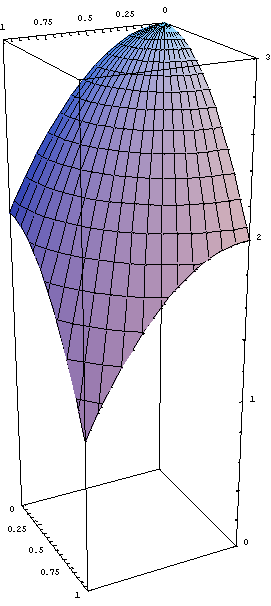
\includegraphics{./images/ch11/volO.pdf}}\quad 
	\resizebox{!}{4.2cm}{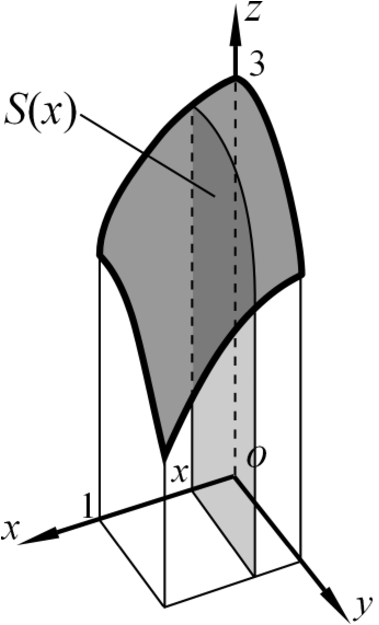
\includegraphics{./images/ch11/volD.pdf}}\quad 
	\resizebox{!}{4.2cm}{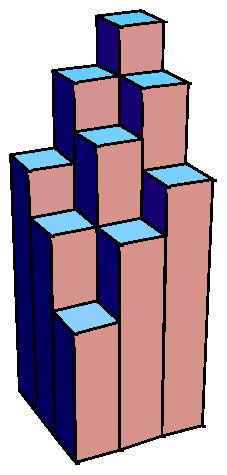
\includegraphics{./images/ch11/volC.pdf}}\quad 
	\resizebox{!}{4.2cm}{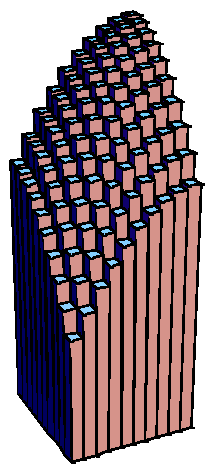
\includegraphics{./images/ch11/volX.pdf}}
\end{center}

[解]:如图,垂直于$x$轴切割该立体,则体积微元
$$\d V=S(x)\d x,\quad x\in([0,1]$$
其中截面积:
$$S(x)=\dint_0^1(3-x^2-y^2)\d y=\df 83-x^2,\quad x\in([0,1]$$

故所求体积
$$V=\dint_0^1S(x)\d x=\df 73$$

对于这类体积问题,看来使用定积分是完全可以的。然而,如果是下面的问题:

{\bf 例:}设以上$\Omega$内部任一点$(x,y,z)$处的密度为$\rho=1+z$,
求$\Omega$的质量。

[分析]:因为$\Omega$是“处处不均匀”的,因此简单由以上的方法就很难求得所要的结果了。


{\bf 定义:}{\it “分割取近似,做和求极限”}
\ps{通过与定积分的类比,理解、记忆重积分的概念与性质}
\begin{enumerate}[(1)]
  \setlength{\itemindent}{1cm}
  \item {\bf 二重积分:} 
  $$\iint_Df(x,y)\d\sigma=\lim_{d(T)\to
  0}\sum_{i=1}^nf(\xi_i,\eta_i)\Delta\sigma_i$$ 
  \item {\bf 三重积分:} 
  $$\iiint_{\Omega}f(x,y,z)\d V=\lim_{d(T)\to
  0}\sum_{i=1}^nf(\xi_i,\eta_i,\zeta_i)\Delta V_i$$
\end{enumerate}

{\bf 基本性质:}\ps{以二重积分为例,但类似的性质同样适用于任意维度的积分}
\begin{enumerate}[(1)]
  \setlength{\itemindent}{1cm}
  \item {\it 线性性}:线性运算可以和重积分交换次序 
  \item {\it 区域可加性} :两个不相重叠的区域上的重积分的和
  等于这个区域的并集上的重积分
  \item {\it 保号性I:} 若在$D$上,$f(x,y)\geq 0$,则
  $$\iint_Df(x,y)\d\sigma\geq 0$$ 
  即:重积分不改变不等号的方向!
  \item {\it 保号性II:} 若$f(x,y)$在$D$上连续,则
  $$\iint_Df(x,y)\d\sigma=0$$
  当且仅当在$D$上恒有$f(x,y)=0$
    \begin{itemize}
	  \item 若在$D$上,$f(x,y)\leq g(x,y)$,则
	  $$\iint_Df(x,y)\d\sigma\leq\iint_Dg(x,y)\d\sigma$$ 
	  \item 推论
	  $$\left|\iint_Df(x,y)\d\sigma\right|\leq\iint_D|f(x,y)|\d\sigma$$ 
	  \item 设$M,m$分别为$f(x,y)$在$D$上的最大和最小值,$D$的面积为$A$,则
	  $$mA\leq\iint_Df(x,y)\d\sigma\leq MA$$
	\end{itemize}
  \item {\it 积分中值定理:}设函数$f(x,y)$在有界闭区域$D$上连续非负,$D$的面积为$A$,则存在
	$(\xi,\eta)\in D$,使得
	$$\iint_Df(x,y)\d\sigma=f(\xi,\eta)A$$
  即:连续函数在有界闭区域上的重积分存在均值点
\end{enumerate}

\section{二重积分的计算}

% {\bf Keyword:}积分次序

重积分的概念实际上给了我们一种进行重积分数值计算(近似计算)的方法,与本节所
介绍的重积分的计算方法并无太大关联。如果说在现代科学中计算与数学已经成为并立
的两大领域,那么重积分的概念与计算也具有这样的关系。

重积分的计算,或者说从代数的角度计算重积分(从而得到精确的代数表示或数值结果),
我们的基本思路是将其转化为一系列相关联(更准确地说,是相互嵌套)的定积分,
然后分步加以处理。因此,其实质还是用定积分来解决问题,只是问题本身的维度更高了。

也正因为如此,接下来的内容是具有较强“技术性”的。

\subsection{在直角坐标系下计算}

$$\iint_Df(x,y)\d\sigma
% =\lim_{d(T)\to0}\sum_{i=1}^nf(\xi_i,\eta_i)\Delta\sigma_i
$$

从抽象形式上看,对积分区域采用平行于$x$轴和$y$轴的直线进行分割,则可以记
面积微元
$$\d\sigma=\d y\d x,$$
其中$\d x$和$\d y$可视为直线间的水平和垂直间距对应的微元(假设分割足够细密)。

另一方面,积分区域可以表示为
$$D=\{x_1\leq x\leq x_2,\varphi_1(x)\leq y\leq \varphi_2(x)\}$$
则二重积分可化为如下的{\it 累次积分:}
$${\iint_Df(x,y)\d\sigma=\int_{x_1}^{x_2}
\int_{\varphi_1(x)}^{\varphi_2(x)}f(x,y)\d y\d x}$$
累次积分是多个定积分的嵌套,按照从内至外的次序进行计算。

{\bf 例:}计算区域
$$D:0\leq x\leq 1,\;x^2\leq y\leq 1$$
的面积。

\begin{center}
	\resizebox{!}{6cm}{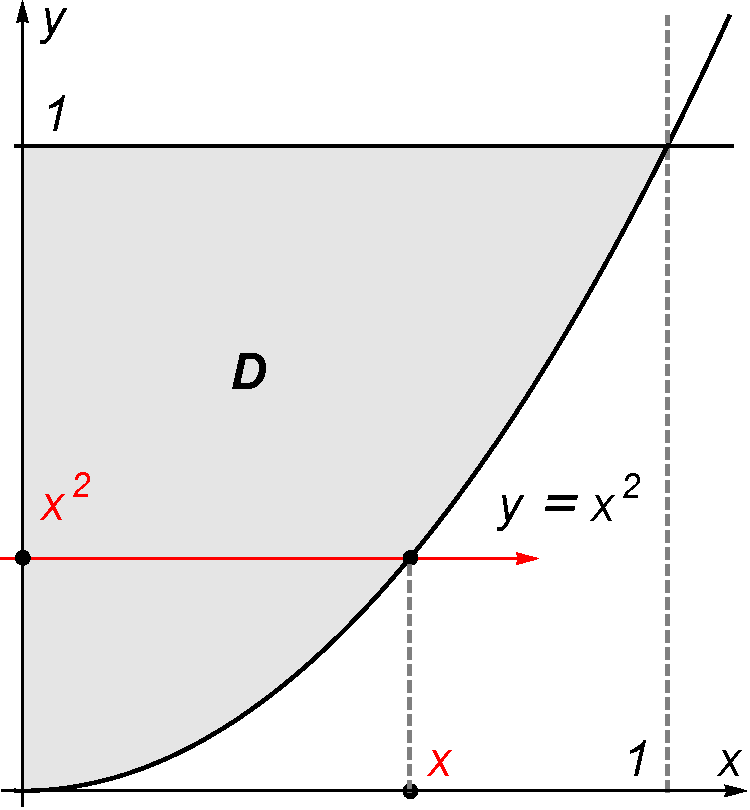
\includegraphics{./images/ch11/2DI-1-1.pdf}}
\end{center}

[解1](定积分)由定积分的几何意义,所求面积
$$S=\dint_0^1(1-x^2)\d x=\df23.$$

[解2](二重积分,先$y$后$x$)如图,由已知,所求面积
$$S=\iint_D\d\sigma=\dint_0^1\dint_{x^2}^1\d y\d x
=\dint_0^1(1-x^2)\d x=\df23.$$

[解3](二重积分,先$x$后$y$)如图,

\begin{center}
	\resizebox{!}{6cm}{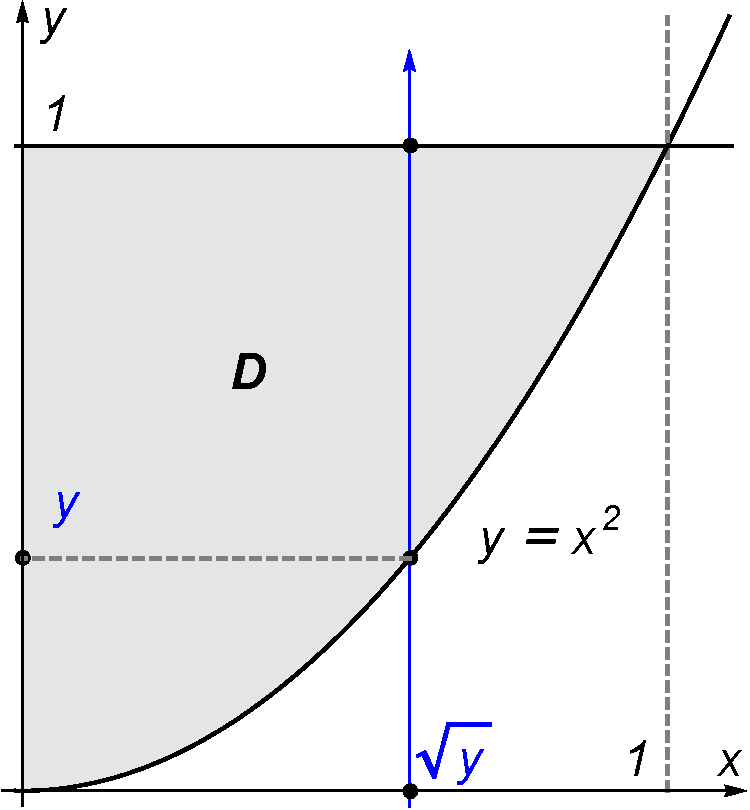
\includegraphics{./images/ch11/2DI-1-2.pdf}}
\end{center}

区域$D$可以表示为
$$D:0\leq y\leq 1,\;0\leq x\leq\sqrt y,$$
故所求面积
$$S=\iint_D\d\sigma=\dint_0^1\dint_0^{\sqrt y}\d x\d y
=\dint_0^1\sqrt y\d y=\df23.$$

{\bf 注:}%关于二重积分的计算
\begin{enumerate}[(1)]
  \setlength{\itemindent}{1cm}
  \item 重积分计算的一般步骤:{\it 画图$\to$定限$\to$积分}
  \item 定限的次序决定了累次积分的次序,且二者正好是相反的
  \item 定限过程(以先$x$后$y$为例)\ps{使用这种描述的意义在于便于向不同的情形推广}
  \begin{enumerate}[Step-1:]
    \setlength{\itemindent}{1cm}
    \item 将积分区域沿着$x$的等值线(也即$x$轴的垂线)方向向$x$轴投影,
    所得区间即为$x$的最大变化范围($[x_1,x_2]$)
    \item 任取$x\in[x_1,x_2]$,作$x$的等值线,自下而上穿过积分区域
    \item 等值线的入射和出射点即为与该$x$值对应的$y$的变化范围,这个
    变化范围一般是和$x$相关的($y_1(x)\leq y\leq y_2(x)$)
  \end{enumerate}
  \item 将二重积分写成累次积分,必须确保{\it 每个累次积分的上限大于下限}。为了便于
  判断各种大小关系,一般需要画图
  \item 计算累次积分,按照从内至外的次序依次进行,计算内层的积分时,外层积分
  的积分变量均视为常数
\end{enumerate}

\begin{shaded}

{\bf 讨论:}二重积分一定比定积分更好吗?

对比上例中不同的解答过程,用定积分的方法最为简明。那么是不是说
使用定积分的方法求解二重积分会比将二重积分化为累次积分计算更好呢?

{\bf 例:}已知面密度$\mu=x^2+y^2$,求区域$D$所对应的平面薄片的质量。

[分析]:如果使用二重积分的方法,则所求质量
$$M=\iint_D(x^2+y^2)\d\sigma.$$
如果使用先$y$后$x$的积分次序,则
$$M=\dint_0^1\dint_{x^2}^1(x^2+y^2)\d y\d x,$$
对于右侧的累次积分,按照从内至外的次序进行计算,计算内层积分时,外层的积分变量($x$)
应视为常数,故
$$M=\dint_0^1\dint_{x^2}^1(x^2+y^2)\d y\d x
=\dint_0^1\left[x^2y+\df13y^3\right]_{x^2}^1\d x=\ldots$$

如果用定积分来计算质量,则需将以上内层的积分视为关于$x$或$y$的函数(视定限的次序),
计算更为复杂。从实际的物理意义上看,也没有二重积分清晰。

事实上,在与平面区域相关的众多应用问题中,使用二重积分的方式
进行求解是更加直观,也比较方便计算的。前上例中,定积分之所以会“显得”
简便,是因为我们考虑的是面积问题(被积函数恒为$1$)。

\end{shaded}
% 
% {\bf 积分区域与累次积分的次序:}
% 将二重积分化为累次积分时,不同的积分次序,对应于不同的积分区域表示方法;或者也可以
% 说,不同的积分区域表示方法,决定了最终的积分次序。

% {\bf 教材-例1:}计算
% $$\iint_Dxy\d\sigma,$$
% 其中$D$为抛物线$y=x^2$和$x=y^2$所围区域。
% 
% \begin{itemize}
%   \setlength{\itemindent}{1cm}
%   \item {先$x$后$y$:}$D:y^2\leq x\leq\sqrt y,\,0\leq y\leq 1$ 
%   \item {先$y$后$x$:}$D:x^2\leq y\leq\sqrt x,\,0\leq x\leq 1$
% \end{itemize}

将二重积分化成累次积分计算,根据累次积分次序的不同,解题过程会有所不同。
通过对题目的分析,选择合适的积分次序,从而使得解题更为简便,是一个重要的技巧。

{\bf 教材-例2:}计算
$$\iint_D\df{x^2}{y^2}\d\sigma,$$
其中$D$由直线$y=2,\,y=x$和$xy=1$围成。

\begin{center}
	\resizebox{!}{6cm}{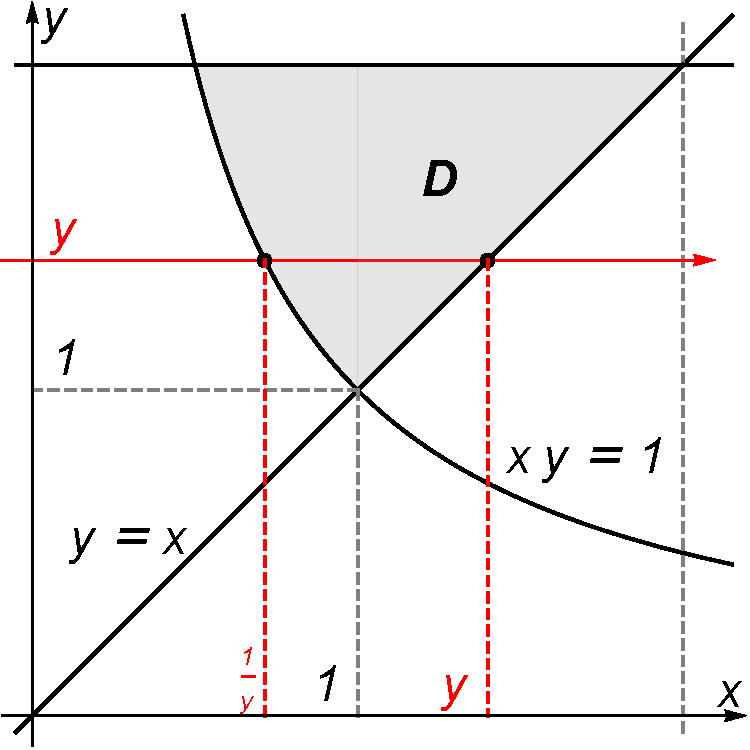
\includegraphics{./images/ch11/2DI-2.pdf}}
\end{center}

[分析]:如图,按照先$y$后$x$的次序定限,可得
$$D:1\leq y\leq 2,\;\df1y\leq x\leq y,$$
从而积分可化为
$$\iint_D\df{x^2}{y^2}\d\sigma
=\dint_1^2\dint_{1/y}^y\df{x^2}{y^2}\d x\d y.$$

如果按先$x$后$y$的次序定限,则如图

\begin{center}
	\resizebox{!}{6cm}{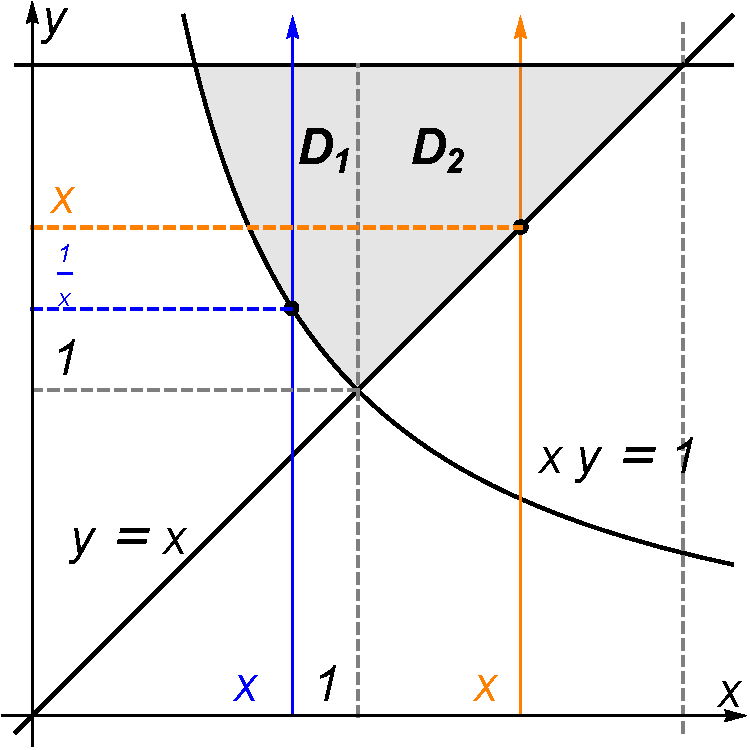
\includegraphics{./images/ch11/2DI-2-1.pdf}}
\end{center}

须将$D$沿$x=1$分割为两个子区域$D_1$和$D_2$,然后分别定限
$$D_1:\df12\leq x\leq 1,\;\df1x\leq y\leq 2,$$
$$D_2:1\leq x\leq 2,\;x\leq y\leq 2,$$
于是,所求积分应改写为
\begin{align*}
	\iint_D\df{x^2}{y^2}\d\sigma&
	\left(\iint_{D_1}+\iint_{D_2}\right)\df{x^2}{y^2}\d\sigma\\
	&=\dint_{1/2}^1\dint_{1/x}^2\df{x^2}{y^2}\d y\d x
	+\dint_1^2\dint_x^2\df{x^2}{y^2}\d y\d x
\end{align*}

{\bf 例:}已知$D:0\leq x\leq 1,1\leq x+y\leq 2$,计算二重积分
$$\iint_D\df1{x+y}\d\sigma$$

{\bf 教材-例3:}计算
$$\iint_D\df{\sin y}{y}\d\sigma,$$
其中$D$由$x=y^2$和$y=x$所围成。

这个例子说明,选择不同的积分次序有时不仅仅是计算是否方便的问题,
甚至可能是能不能计算的问题。

{\bf 教材-例5:}计算累次积分
$$I=\int_{1/4}^{1/2}\int_{1/2}^{\sqrt y}e^{y/x}\d x\d y+
\int_{1/2}^1\int_y^{\sqrt y}e^{y/x}\d x\d y$$

累次积分交换积分次序是非常典型的一类题目。需要注意的是,并不是每个累次积分
都可以直接改写成二重积分,例如:
$$\dint_0^{2\pi}\dint_0^{\sin x}f(x,y)\d y\d x$$
由于内层积分不能确定总是上限大于下限,因此不能简单地将其化成{\it 一个}二重积分。

{\bf 教材-例4:}求两柱面$x^2+y^2=R^2,\, x^2+z^2=R^2$
相交所围成的立体体积。

\begin{center}
% 	\resizebox{!}{5cm}{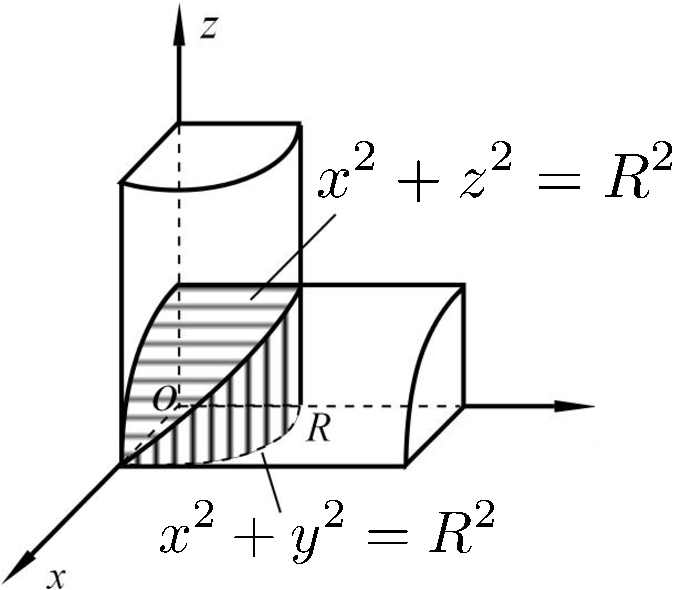
\includegraphics{./images/ch11/intersectV.pdf}}
	\resizebox{!}{6cm}{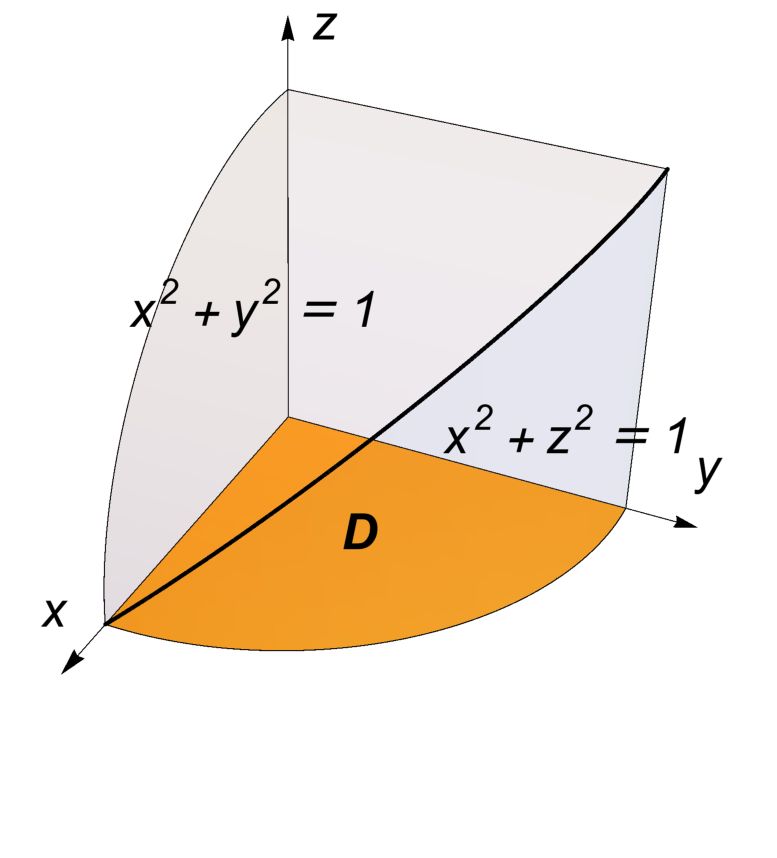
\includegraphics{./images/ch11/3DI-1.pdf}}
\end{center}

\subsection{在极坐标系下计算}

有时候积分区域在直角坐标系下进行定限,没有在极坐标系下那么方便。

{\bf 例:}已知区域$D$为单位圆的右半部分,求
$$\iint_D(x^2+y^2)\d\sigma$$

[分析]:区域$D$可表示为
$$D:\;0\leq x\leq 1,\;-\sqrt{1-x^2}\leq y\leq\sqrt{1-x^2}.$$
故
\begin{align*}
	\iint_D(x^2+y^2)\d\sigma
	&=\dint_0^1\dint_{-\sqrt{1-x^2}}^{\sqrt{1-x^2}}(x^2+y^2)\d y\d x\\
	&=\dint_0^1\left[2x^2\sqrt{1-x^2}+\df13(1-x^2)^{3/2}\right]\d x\\
	&=\ldots
\end{align*}
定限的结果繁琐,导致积分的计算也比较复杂。

之所以会这样,因为采用垂直、水平的直线对区域进行分割、定限,对于圆弧围成的区域,
远不如对矩形那么简便。

使用极坐标变换计算二重积分,主要适用于边界包含圆弧(准确地说是以原点为圆心的圆弧)
的区域。例如该例中的积分区域完全可以表示成:
$$D:\;-\df{\pi}2\leq\theta\leq\df{\pi}2,
\;0\leq\rho\leq1.$$

如果扩展矩形的定义为由变量的{\it 等值线}——也即在该曲线上对应变量的值不变——所围成的区域,
那么类似以上的区域即为极坐标系下的“矩形”。对任何一种坐标系来说,矩形都是最
容易定限的积分区域。

在极坐标系下,一般的“矩形”形如下图:

\begin{center}
	\resizebox{!}{5cm}{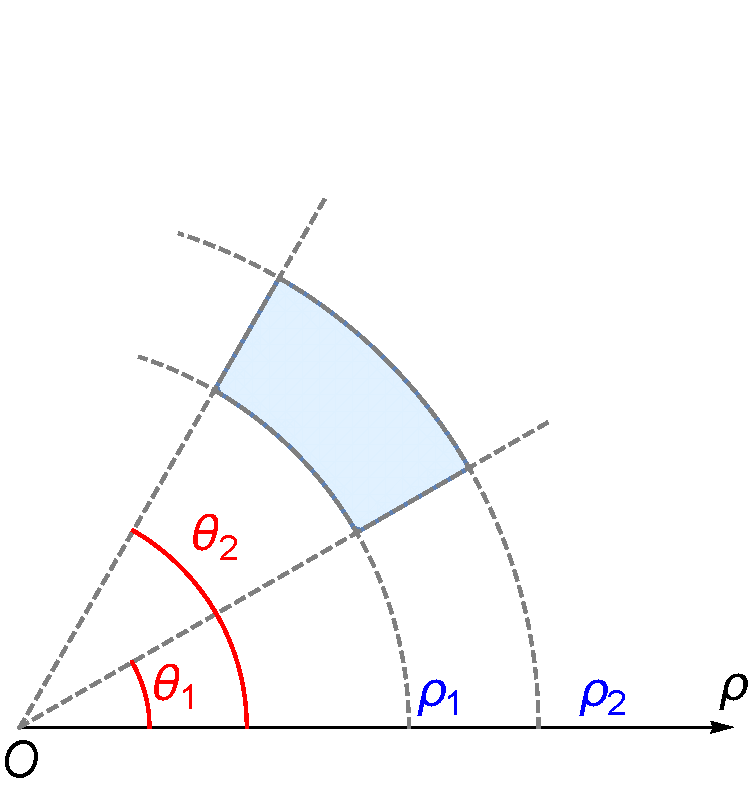
\includegraphics{./images/ch11/PolarRectangle.pdf}}
\end{center}

阴影部分分别由$\rho$的等值线$\rho=\rho_1,\rho=\rho_2$和$\theta$的
等值线$\theta=\theta_1,\theta=\theta_2$围成。

{\bf 思考:}极坐标系下的“矩形”有哪些可能的形状?

相应地,极坐标系下的面积微元也采用$\rho$和$\theta$的等值线分割而成,形如下图:

\begin{center}
	\resizebox{!}{5cm}{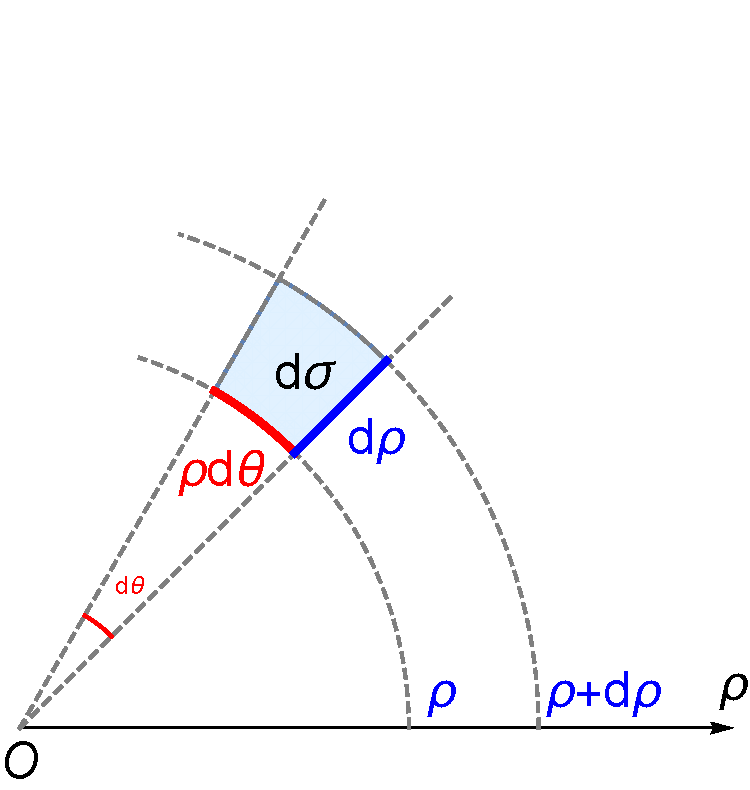
\includegraphics{./images/ch11/PolarDD.pdf}}
\end{center}

将其近似地视为矩形,从而可得
$$\d\sigma=\rho\d\rho\d\theta\quad
\mbox{或}\quad\d\sigma=\rho\d\theta\d\rho$$

于是,根据定限的不同结果,可得在极坐标系下计算二重积分的公式为

\begin{align*}
	\iint_Df(x,y)\d\sigma
	&=\int_{\theta_1}^{\theta_2}\int_{\rho_1(\theta)}^{\rho_2(\theta)}
	f(\rho\cos\theta,\rho\sin\theta)\rho \d\rho \d\theta\\
	&=\int_{\rho_1}^{\rho_2}\int_{\theta_1(\rho)}^{\theta_2(\rho)}
	f(\rho\cos\theta,\rho\sin\theta)\rho\d\theta\d\rho 
\end{align*}

其中的定限方式如下图:

\begin{center}
	\resizebox{!}{4.2cm}{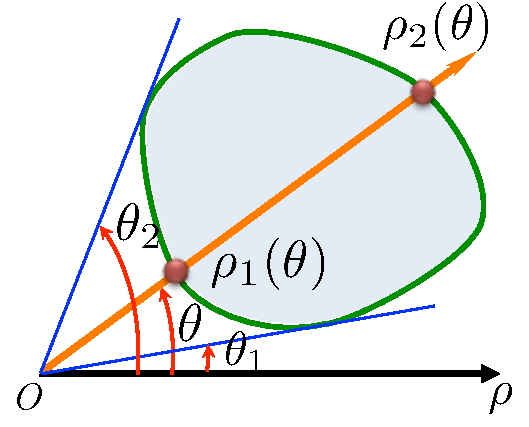
\includegraphics{./images/ch11/tr.pdf}}\hspace{2cm}
	\resizebox{!}{4.2cm}{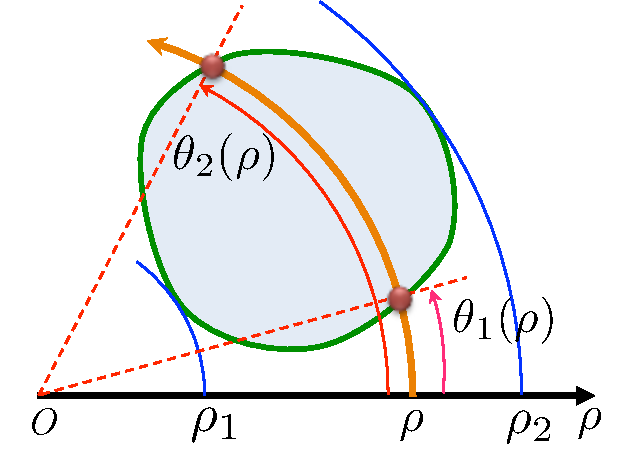
\includegraphics{./images/ch11/rt.pdf}}
	
	$D:\theta_1\leq\theta\leq\theta_2,\rho_1(\theta)\leq\rho\leq\rho_2(\theta)$
	\hspace{2cm}
	$D:\rho_1\leq\rho\leq\rho_2,\theta_1(\rho)\leq\theta\leq\theta_2(\rho)$
\end{center}

以先定$\theta$后定$\rho$为例,过程可以描述如下:\ps{注意理解等值线的意义:坐标变换的
主要目的就是利用变换后新变量的等值线,实现对积分区域更好的切割,从而便于定限}

\begin{enumerate}[Step-1:]
  \setlength{\itemindent}{1cm}
  \item 将积分区域沿着$\theta$的等值线(从原点出发的射线)方向投影到单位圆上,其中得到的
  弧长范围即为$\theta$对应的最大变化范围($[\theta_1,\theta_2]$)
  \item 任取$\theta\in[\theta_1,\theta_2]$,从原点出发作$\theta$的等值线穿过积分区域
  \item 等值线的入射点和出射点对应的$\rho$值即为与选定的$\theta$值相对应的$\rho$的
  变化范围($[\rho_1(\theta),\rho_2(\theta)]$)
\end{enumerate}

在极坐标系下,前述例题的解题过程:

[解]:令$x=\rho\cos\theta,y=\rho\sin\theta$,在极坐标系下:
$$D:\;-\df{\pi}2\leq\theta\leq\df{\pi}2,
\;0\leq\rho\leq1.$$
故
$$\iint_D(x^2+y^2)\d\sigma
=\dint_{-\pi/2}^{\pi/2}\dint_0^1\rho^2\rho\d\rho\d\theta
=\df{\pi}4
$$

过程大大简化了。

{\bf 例:}计算二重积分
$$\iint_D(x^2+y^2)\d x\d y,$$
其中$D$由圆$x^2+y^2=2y,\,x^2+y^2=4y$及直线
$x=\sqrt 3y,\,y=\sqrt 3x$围成。

{\bf 教材-例1:}计算二重积分
$$\iint_D\arctan\df yx\d\sigma,$$
其中$D$为双扭线
$$(x^2+y^2)^2=a^2(x^2-y^2)\;(a>0)$$
与$x$轴正向围成图形在第一象限中的部分。

\begin{center}
	\resizebox{!}{4.5cm}{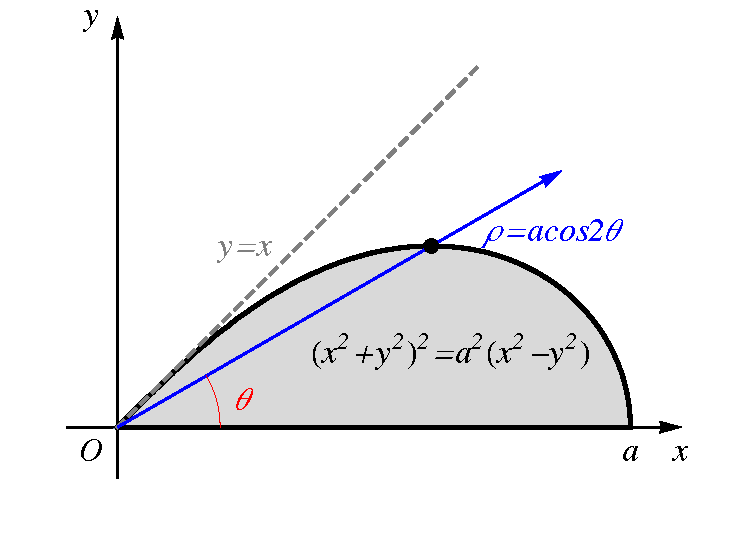
\includegraphics{./images/ch11/2TwistRT.pdf}}
\end{center}

{\bf 例:}求球体$x^2+y^2+z^2\leq 4a^2$包含在圆柱$x^2+y^2=2ax\,(a>0)$
内的体积。

\begin{center}
	\resizebox{!}{5cm}{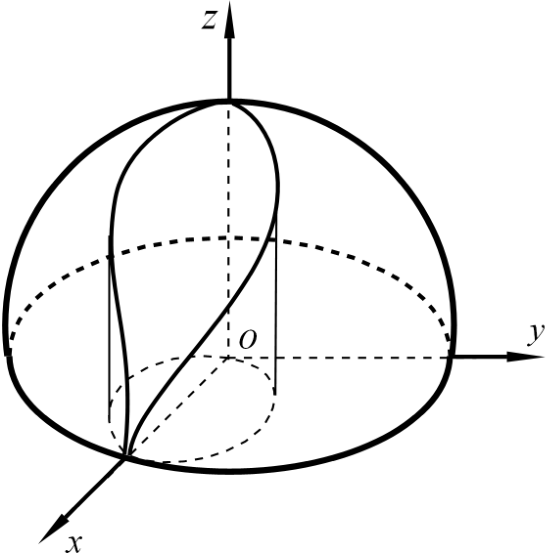
\includegraphics{./images/ch10/viviani.pdf}}
\end{center}

{\bf 教材-例2:}计算椭圆抛物面$z=x^2+2y^2$与抛物柱面$z=2-x^2$所围成
的立体体积。

\begin{center}
	\resizebox{!}{5cm}{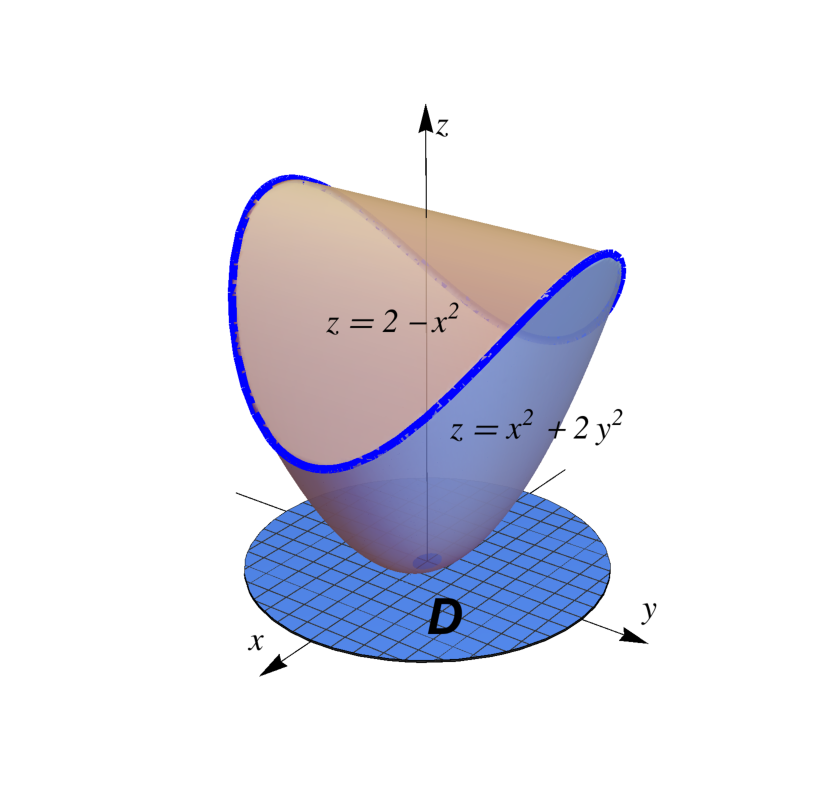
\includegraphics{./images/ch11/surface-ud.pdf}}
\end{center}

{\bf 教材-例4:}计算
$$\iint_De^{-x^2-y^2}\d x\d y,$$
其中$D:x^2+y^2\leq a^2$。利用该计算结果求
$$\dint_{-\infty}^{+\infty}e^{-x^2}\d x.$$

\begin{shaded}
	{\bf 一般形式的坐标变换与重积分}
	
	设$f(x,y)$在区域$D\subset\mathbb{R}^2(x,y)$上连续,坐标变换
	$$T:\;x=x(u,v),\;y=y(u,v)$$
	满足:
	\begin{enumerate}[(1)]
	  \item $T$将区域$D'\subset\mathbb{R}^2(u,v)$一一映射为$D$
	  \item $x(u,v),y(u,v)$在$D'$上一阶偏导连续
	  \item 对任意$(u,v)\in D'$,总有
	  $$J(u,v)=\df{\p(x,y)}{\p(u,v)}=\left|\begin{array}{cc}
	  	x'_u & x'_v \\ y'_u & y'_v
	  \end{array}\right|\ne 0$$
	\end{enumerate}
	则
	$$\iint_Df(x,y)\d x\d y=\iint_{D'}f[x(u,v),y(u,v)]|J(u,v)|\d u\d v$$
	
	{\bf 注:}关于Jacobi行列式,具有如下的性质
	$$\left|\begin{array}{cc}
	  	x'_u & x'_v \\ y'_u & y'_v
	  \end{array}\right|
	  =\left|\begin{array}{cc}
	  	u'_x & u'_y \\ v'_x & v'_y
	  \end{array}\right|^{-1}$$
\end{shaded}

\subsection{对称性的应用}

{\bf 例:}已知$D:0\leq x\leq1,0\leq y\leq1$,计算二重积分
$$\iint_D(x+y)\mathrm{sgn}(x-y)\d\sigma$$

通过本例体会对称性在重积分计算中的应用。进而推广得到如下命题:

{\bf 定理:}已知区域$D$关于直线$L$对称,若对任意关于$L$对称的两点
$P$、$Q$,总有
$$f(P)=-f(Q),$$
则
$$\iint_Df(x,y)\d\sigma=0.$$

又若$D_1$表示区域$D$位于$L$一侧的子区域,且
$$f(P)=f(Q),$$
则
$$\iint_Df(x,y)\d\sigma=2\iint_{D_1}f(x,y)\d\sigma.$$

该定理有一些常用的推论:

{\bf 推论:}设区域$D$关于$x=0$对称,且对任意$(x,y)\in D$,有
\ps{可称之为$f$是关于$x$的奇函数}
$$f(x,y)=-f(-x,y),$$
则
$$\iint_Df(x,y)\d\sigma=0.$$

又若$D_1$表示$D$中对应$x\geq0$的子区域,且
$$f(x,y)=f(-x,y),$$
则
$$\iint_Df(x,y)\d\sigma=2\iint_{D_1}f(x,y)\d\sigma.$$

{\bf 例:}$D:x^2+y^2\leq 1$,不难验证
$\ds\iint_D\df{3x-4\sin y}{x^2+2y^2}\d\sigma=0$

{\bf 推论:}设区域$D$关于$y=x$对称,且对任意$(x,y)\in D$,有
$$f(x,y)=-f(y,x),$$
则
$$\iint_Df(x,y)\d\sigma=0.$$

{\bf 例:}$$\iint_{x^2+y^2\leq 1}\df{(x+2y)^2}{1+x^2+y^2}d\sigma$$

{\bf 定理:}设区域$D_1$和$D_2$关于$y=x$对称,则
$$\iint_{D_1}f(x,y)\d\sigma=\iint_{D_1}f(y,x)\d\sigma.$$

{\bf 推论}(轮换对称性)设区域$D$关于$y=x$对称,则
$$\iint_Df(x,y)\d\sigma=\iint_Df(y,x)\d\sigma.$$

{\bf 例:}区域$D$为第一象限内的四分之一单位圆,求
$$\iint_D\df{2x^2+x-y+1}{\sqrt{1-x^2-y^2}}d\sigma$$

% {\bf 例:}设$D:\df{x^2}{a^2}+\df{y^2}{b^2}\leq1$,求
% $$\iint_D(x+y)^2\d\sigma$$

{\bf 例:}区域$D$为第一象限内半径为$2$的圆,$f(x)$恒不为零,求
$$\iint_D\df{\sqrt{f(x)}}{\sqrt{f(x)}+\sqrt{f(y)}}d\sigma$$

{\bf 思考:}若该例子中的区域改为椭圆$\df{x^2}{a^2}+\df{y^2}{b^2}\leq 1$,
结果会怎样?

\section{三重积分的计算}

\subsection{在直角坐标系下计算}

$${I=\iiint_{\Omega}f(x,y,z)\d V}$$

如果说二重积分的计算思路是把“$2$”化成“$1+1$”形式的定积分,那么三重积分显然就应该
是先将“$3$”化成“$1+2$”或者“$2+1$”,然后将其中的$2$分解为“$1+1$”,最终得到
可以分步加以计算的“$1+1+1$”。

\begin{enumerate}
  \item {\bf 微元法(投影法):}
  $$I=\iint_D\int_{z_1(x,y)}^{z_2(x,y)}f(x,y,z)\d z\d\sigma$$
  \item {\bf 截面法:}
  $$I=\int_{z_1}^{z_2}\iint_{D(z)}f(x,y,z)\d\sigma \d z$$
\end{enumerate}

\subsubsection{【微元法(投影法)】}

设$\Omega$在$xOy$平面上的投影区域为$D$, $\d V=\d z\d\sigma$, 
\ps{先投影,再定$z$,化成“2+1”}
$$\Omega=\{z_1(x,y)\leq z\leq z_2(x,y), (x,y)\in D\}$$

\begin{center}
	\resizebox{!}{4.5cm}{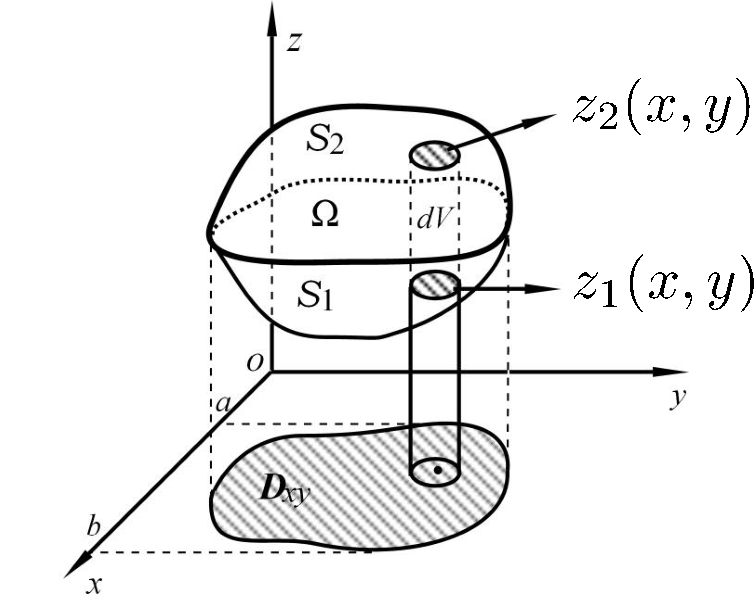
\includegraphics{./images/ch11/DxyZ.pdf}} 
\end{center}

$${I=\iiint_{\Omega}f(x,y,z)\d
V=\iint_D\int_{z_1(x,y)}^{z_2(x,y)}f(x,y,z)\d z\d\sigma}$$

\subsubsection{【截面法】}

取$\Omega$的水平截面,其在$xOy$平面上的投影区域为$D(z)$,
$\d V=\d\sigma \d z$,\ps{先定$z$,再投影,化成“1+2”}
$$\Omega=\{(x,y)\in D(z),z_1\leq z\leq z_2\}$$

\begin{center}
	\resizebox{!}{4.5cm}{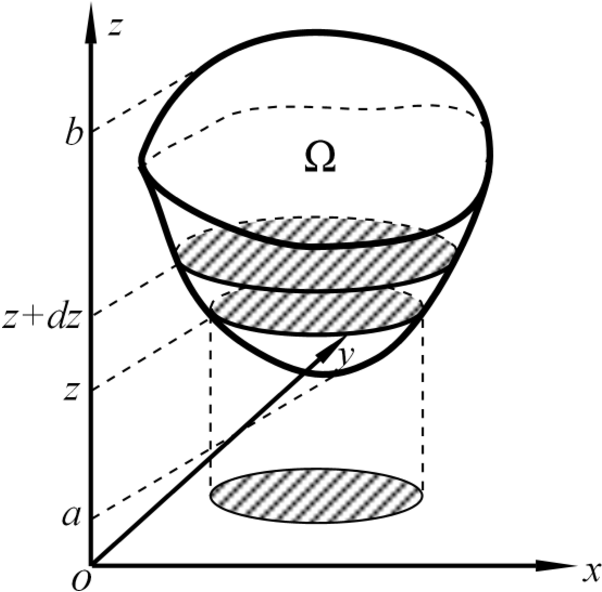
\includegraphics{./images/ch11/Dzxy.pdf}}
\end{center}

$${I=\iiint_{\Omega}f(x,y,z)\d
V=\int_{z_1}^{z_2}\iint_{D(z)}f(x,y,z)\d\sigma \d z}$$

{\bf 教材-例7:}计算三重积分
$$I=\iiint_{\Omega}\df1{(1+x+y+z)^3}\d V,$$
其中$\Omega$为平面$x+y+z=1$与三个坐标面所围成的空间区域。

\begin{center}
	\resizebox{!}{6cm}{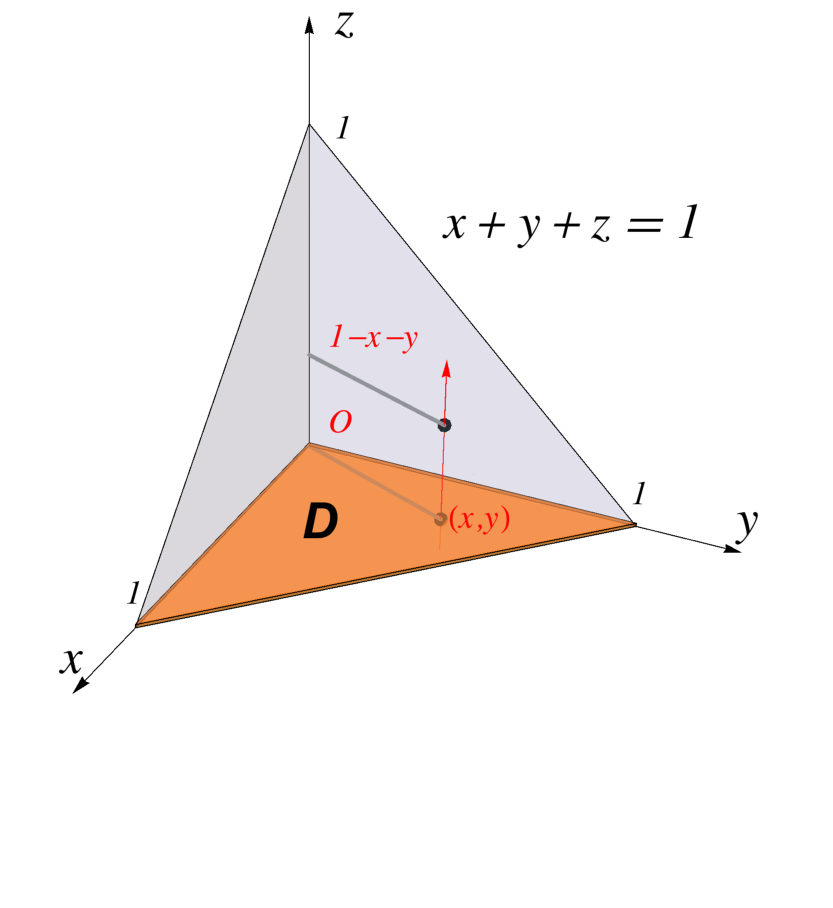
\includegraphics{./images/ch11/3DTri21.pdf}} 
	\resizebox{!}{6cm}{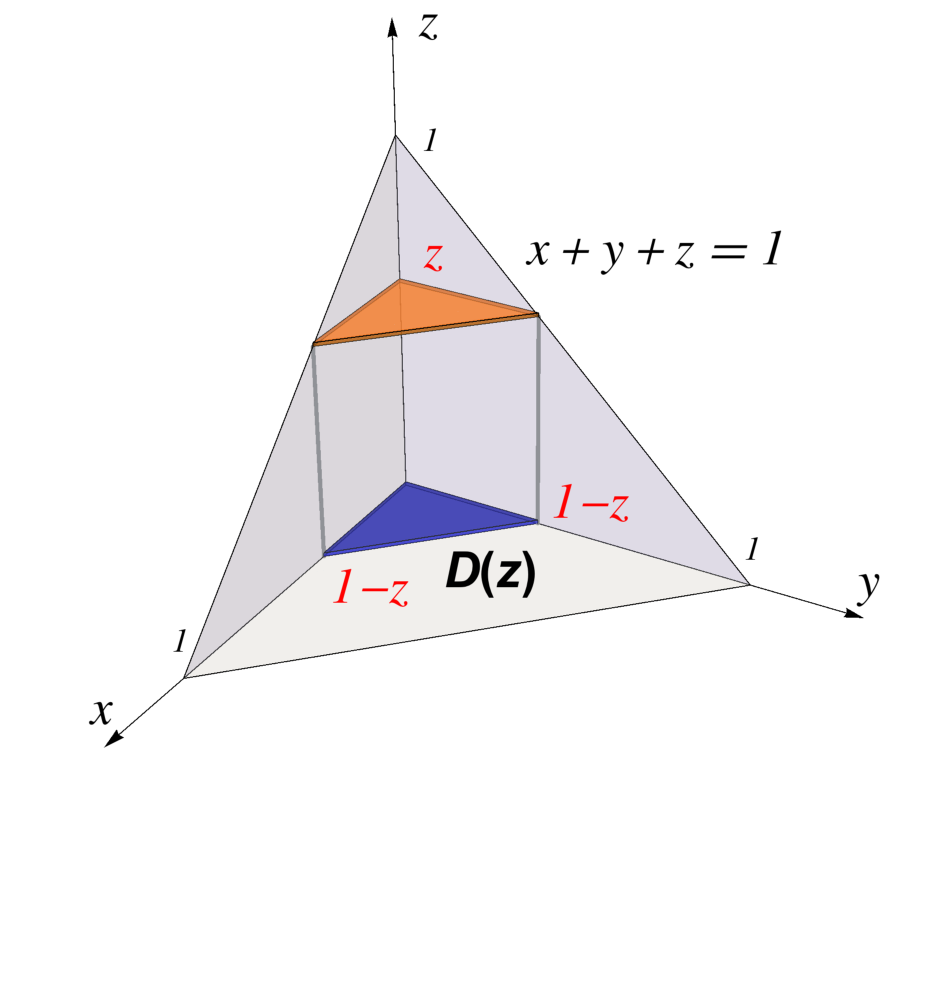
\includegraphics{./images/ch11/3DTri12.pdf}} 
\end{center}

[分析]:采用两种不同的定限方法,所得结果分别为
$$\Omega:(x,y)\in D,\;0\leq z\leq 1-x-y$$
$$\Omega:-1\leq z\leq 1,(x,y)\in D(z)$$
进而得到
$$\Omega:0\leq x\leq 1,\;0\leq y\leq 1-x,\;0\leq z\leq 1-x-y$$
$$\Omega:0\leq z\leq 1,\;0\leq x\leq 1-z,\;0\leq y\leq 1-z-x$$
对应的累次积分别为
$$\dint_0^1\dint_0^{1-x}\dint_0^{1-x-y}\df1{(1+x+y+z)^3}\d x\d y\d z$$
$$\dint_0^1\dint_0^{1-z}\dint_0^{1-z-x}\df1{(1+x+y+z)^3}\d z\d x\d y$$


{\bf 例:}计算三重积分
$$I=\iiint_{\Omega}z^2\d V,$$
其中$\Omega:\df{x^2}{a^2}+\df{y^2}{b^2}+\df{z^2}{c^2}\leq 1$。

\begin{center}
	\resizebox{!}{5cm}{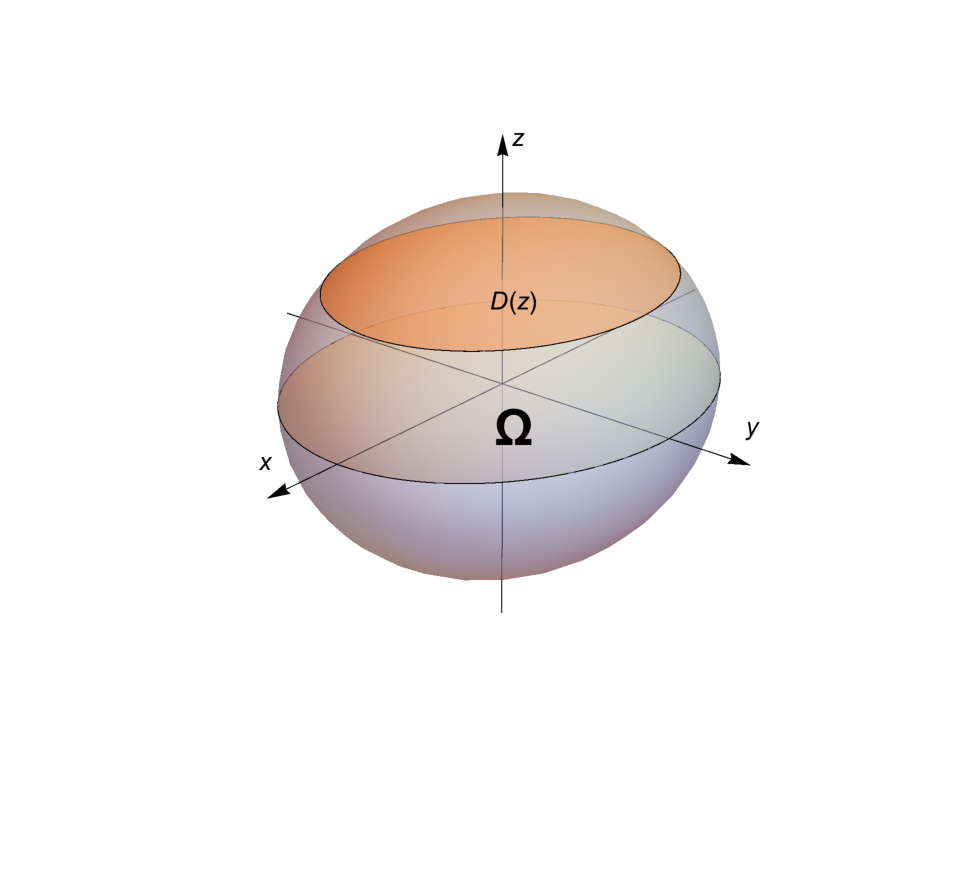
\includegraphics{./images/ch11/3DI-2.pdf}}
\end{center}

{\bf 注:}{\b 如果被积函数只与$z$(或者,准确地说,只与一个变量)有关,
推荐使用截面法!}

{\bf 教材-例8:}将三重积分
$$I=\iiint_{\Omega}f(x,y,z)\d V,$$
化为累次积分,其中$\Omega$为曲面$z=1-x,y=1-z^2$及三个坐标平面所围空间闭区域。

{\bf 教材-例9:}计算三重积分
$$I=\iiint_{\Omega}(x+y+2z)\d V,$$
其中$\Omega$为球体$x^2+y^2+z^2\leq R^2\,(R>0)$在第一卦限中的部分。

{\bf 思考题:}讨论数列$a_n=\ds\iiint_{\Omega_n}z^n\d V$的敛散性,其中
$\Omega_n$由$(x^2+y^2+z^2)^n=a^{2n-1}z\;(a>0)$所围。\hfill $a\in(0,1]$收敛;
反之发散。

\subsection{在柱坐标下计算}

{\bf 从直角坐标到柱坐标:}$M:\;(x,y,z)\;\to(\rho,\theta,z)$,其中
$$x=\rho\cos\theta,\;y=\rho\sin\theta,\;z=z\quad (\rho\geq 0,0\leq\theta\leq
2\pi,z\in\mathbb{R})$$

\begin{center}
	\resizebox{!}{5cm}{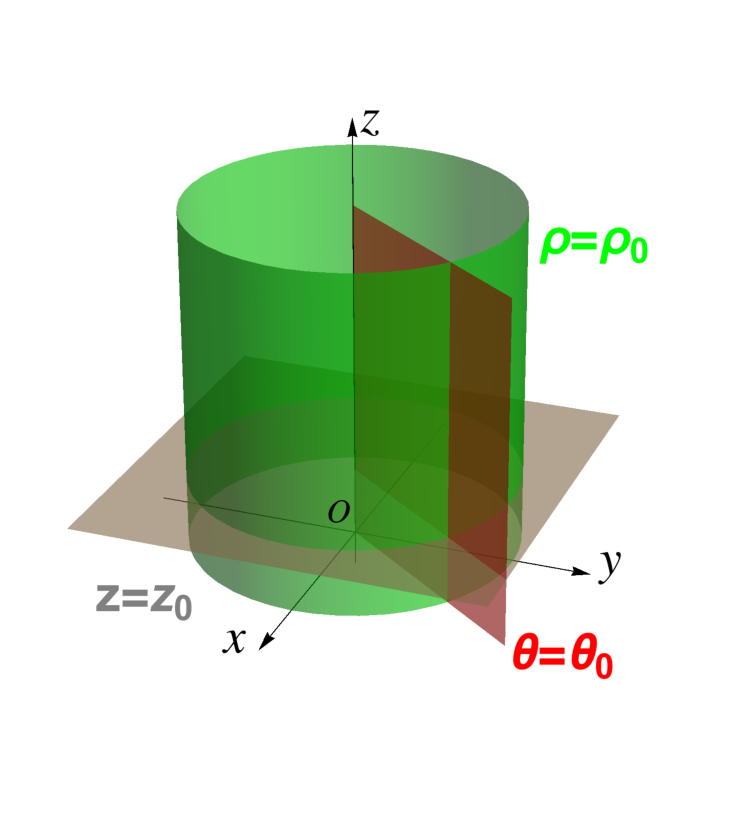
\includegraphics{./images/ch11/cylinCs.pdf}}
	\quad
	\resizebox{!}{5cm}{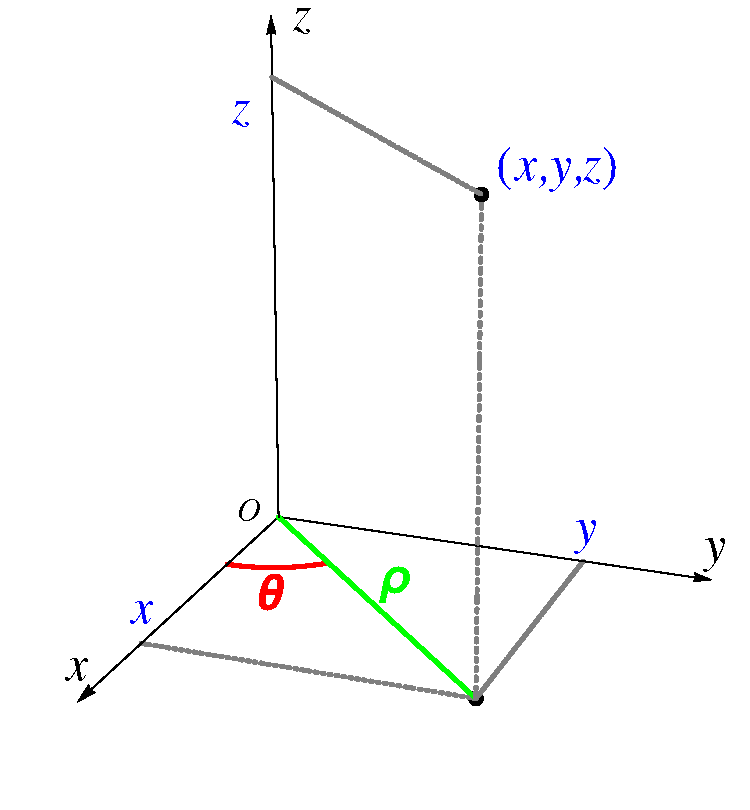
\includegraphics{./images/ch11/cylinCT.pdf}}
\end{center}

柱坐标系下的体积微元

\begin{center}
	\resizebox{!}{5cm}{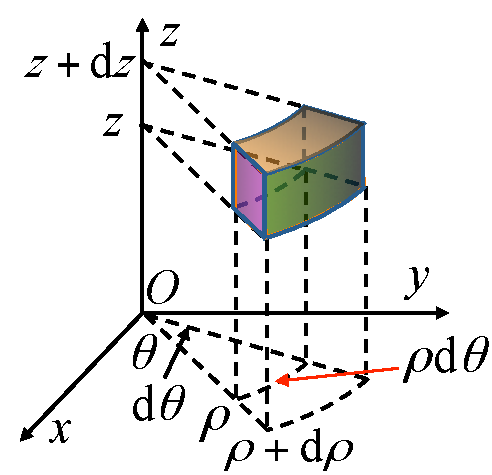
\includegraphics{./images/ch11/polarCy.pdf}}
	$$\d V=\rho \d\rho \d\theta \d z$$
\end{center}

$${\iiint_{\Omega}f(x,y,z)\d
V=\iiint_{\Omega}f(\rho\cos\theta,\rho\sin\theta,z)\rho 
\d\rho \d\theta \d z}$$

微元的表示(微元法)

\begin{center}
	\resizebox{!}{6cm}{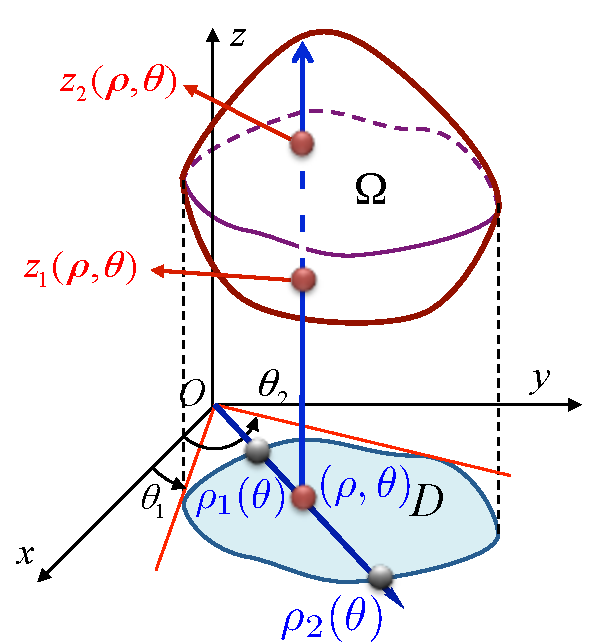
\includegraphics{./images/ch11/cy21.pdf}}
\end{center}

$$\theta_1\leq\theta\leq\theta_2,\;
\rho_1(\theta)\leq\rho\leq\rho_2(\theta),\;
z_1(\rho,\theta)\leq z\leq z_2(\rho,\theta)$$

{\bf 教材-例6:}计算三重积分
$$\iiint_{\Omega}z\sqrt{x^2+y^2}\d V,$$
其中$\Omega$为柱面$x^2+y^2=2x\,(y>0)$与平面
$z=0,\,z=h\,(h>0)$所围立体。

{\bf 例:}计算三重积分
$$\iiint_{\Omega}\df 1{1+x^2+y^2}\d V,$$
其中$\Omega$由$x^2+y^2=4z$与$z=h\,(h>0)$所围成。

{\bf 例:}计算三重积分
$$\iiint_{\Omega}z\d V,$$
其中$\Omega$由$z=x^2+y^2$和$z=4$所围。

[解]:在柱坐标系下,积分区域可表示为
$$\Omega:\;0\leq\theta\leq2\pi,\;0\leq\rho\leq2,\;\rho^2\leq z\leq4,$$
故
$$\iiint_{\Omega}z\d V=
\dint_0^{2\pi}\dint_0^2\dint_{\rho^2}^4z\rho\d z\d\rho\d\theta
=\df{64}3\pi$$

\subsection{在球坐标下计算}

{\bf 直角坐标到球坐标:}$M:\;(x,y,z)\;\to(r,\theta,\varphi)$,其中
$$x=r\sin\varphi\cos\theta,\;y=r\sin\varphi\sin\theta,\;z=r\cos\varphi
\quad(r\geq 0,0\leq\theta\leq 2\pi,0\leq\varphi\leq\pi)$$

\begin{center}
	\resizebox{!}{5cm}{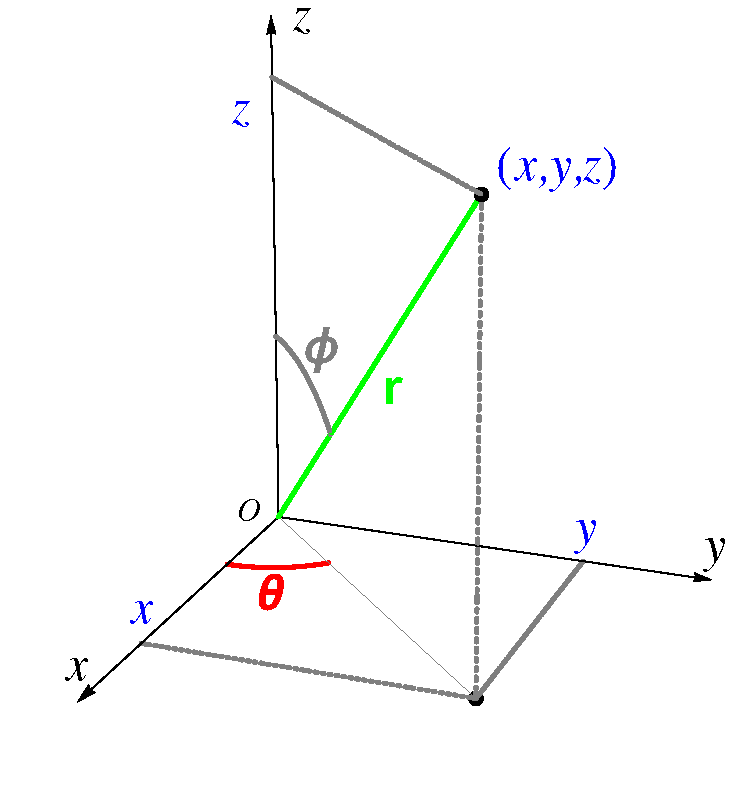
\includegraphics{./images/ch11/sphereXYZ.pdf}}
	\quad
	\resizebox{!}{5cm}{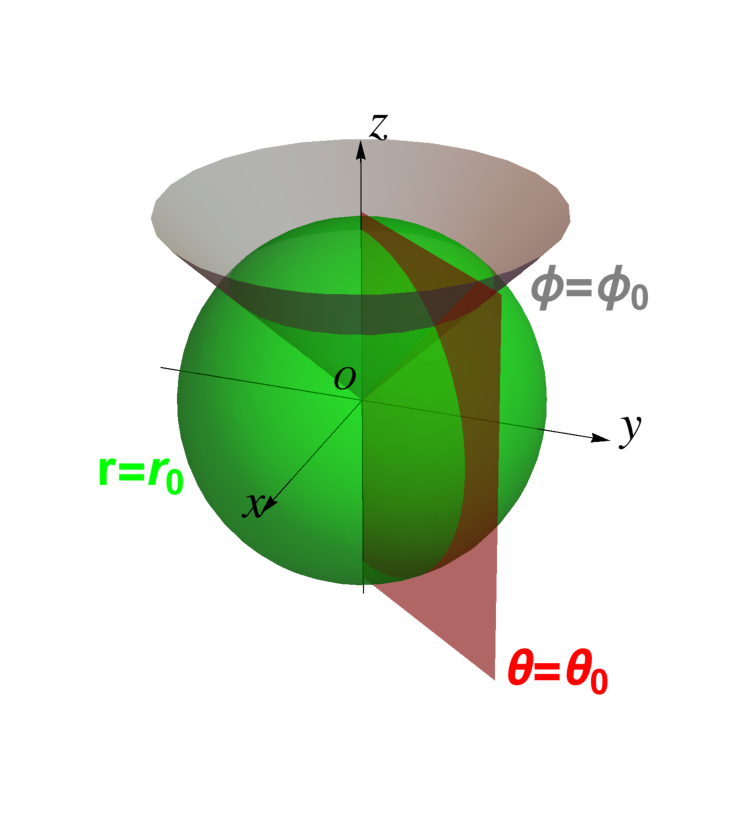
\includegraphics{./images/ch11/sphereEL.pdf}}
\end{center}

球坐标系下的体积微元

\begin{center}
	\resizebox{!}{5.5cm}{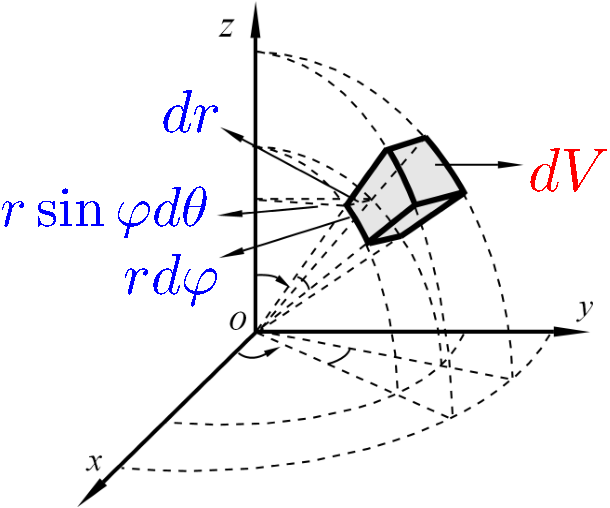
\includegraphics{./images/ch11/sphDv.pdf}} 
\end{center}

$$\d V=r^2\sin\varphi \d r\d\theta \d\varphi$$

{\bf 例:}推导球的体积公式。

{\bf 教材-例7:}计算三重积分
$$\iiint_{\Omega}(x^2+y^2+z^2)\d V,$$
其中$\Omega$由$z=\sqrt{x^2+y^2}$与$x^2+y^2+z^2=R^2$所围成。

{\bf 教材-例8:}计算三重积分
$$\iiint_{\Omega}(x^2+y^2)\d V,$$
其中$\Omega$由$x^2+y^2+z^2=2az$与$x^2+y^2+z^2=2bz$所围成$(0<a<b)$。

{\bf 例:}求半径为$a$的球面与半顶角为$\alpha$的内接锥面所围成的立体体积。

[提示]:在球坐标系下定限:
$$\Omega:\;0\leq\theta2\pi,\;0\leq\phi\leq\alpha,\;0\leq r\leq2a\cos\theta,$$
故所求体积
$$V=\dint_0^{2\pi}\dint_0^{\alpha}\dint_0^{2a\cos\phi}r^2\sin^2\phi\d r
=\df{4\pi a^3}3(1-\cos^4\alpha)$$

\section{重积分的应用}

\subsection{质量}

{\bf P218-例1:}设一平面三角形薄片以$O(0,0),A(1,0),B(0,1)$为顶点,
其上任一点$(x,y)$处的面密度$\mu(x,y)=x^2+y^2$,
求该平面薄片的质量。

\subsection{质心(重心、形心)}

{\bf 空间$n$个质点的质心:}
	
空间中$n$个质点($k=1,2,\ldots,n$),质量分别为$m_k$,坐标$(x_k,y_k,z_k)$
$${\bar{x}=\df{\sum\limits_{k=1}^nx_km_k}{\sum\limits_{k=1}^nm_k},}\;
{\bar{y}=\df{\sum\limits_{k=1}^ny_km_k}{\sum\limits_{k=1}^nm_k},}\; 
{\bar{z}=\df{\sum\limits_{k=1}^nz_km_k}{\sum\limits_{k=1}^nm_k}}$$

{\bf 平面薄片的质心:} 密度函数$\mu(x,y)$,$(x,y)\in D$
$${\bar{x}=\df{\displaystyle\iint_Dx\mu(x,y)\d\sigma}
{\displaystyle\iint_D\mu(x,y)\d\sigma},\;} 
{\bar{y}=\df{\displaystyle\iint_Dy\mu(x,y)\d\sigma}
{\displaystyle\iint_D\mu(x,y)\d\sigma}}$$

{\bf 教材-例4}
设半径为$R$的半圆形薄片上每一点的面密度与该点到圆心的距离成正比,
求该薄片的质心。

{\bf 空间物体的质心:} 密度函数$\mu(x,y,z)$,$(x,y,z)\in\Omega$
$$\bar{x}=\df{\displaystyle\iiint_{\Omega}x\mu(x,y,z)\d V}
{\displaystyle\iiint_{\Omega}\mu(x,y,z)\d V},\;
{\bar{y}=\df{\displaystyle\iiint_{\Omega}y\mu(x,y,z)dV}
{\displaystyle\iiint_{\Omega}\mu(x,y,z)dV},\;} $$
$${\bar{z}=\df{\displaystyle\iiint_{\Omega}z\mu(x,y,z)dV}
{\displaystyle\iiint_{\Omega}\mu(x,y,z)dV}}
$$
{\bf 教材-例6:}求均匀半球壳$\Omega:a^2\leq x^2+y^2+z^2\leq b^2$,
$(0<a<b)$,$z\geq 0$的形心。

\subsection{转动惯量}

{\bf 空间一质点的转动惯量:}$${I=mr^2}$$

\begin{center}
	\resizebox{!}{4cm}{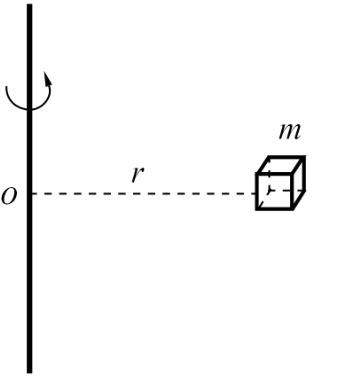
\includegraphics{./images/ch11/roll.pdf}}
\end{center}

{\bf 空间物体绕$z$轴旋转:}密度函数$\mu(x,y,z),(x,y,z)\in\Omega$
$${I=\iiint_{\Omega}(x^2+y^2)\mu(x,y,z)\d V}$$

{\bf 例:}求半径为$R$的均匀半圆形薄片绕其平分线转动的转动惯量和旋转半径。

{\bf 教材-例8:}(平行轴定理)设$L_c$为通过物体$\Omega$质心的直线,直线$L_t$平行于$L_c$,
两者距离为$d$。试证:$\Omega$关于轴$L_t$的转动惯量$I_t$与物体关于轴
$L_c$的转动惯量$I_c$之间存在关系如下:
$$I_t=I_c+Md\,^2,$$
其中$M$为$\Omega$的质量。

{\bf 例:}\ps{同济}求半径为$R$密度为$\mu$的球体绕其直径的转动惯量。

[提示]:不妨以$z$轴为转动轴,则
\begin{align*}
	I_z&=\iiint_{\Omega}(x^2+y^2)\mu\d V\\
	&=\mu\dint_0^{2\pi}\dint_0^{\pi}\dint_0^Rr^4\sin^3\phi\d r
	\d\phi\d\theta\\
	&=\df8{15}\pi\mu R^5
\end{align*}

\subsection{万有引力}

已知占据空间趋于$\Omega$的物体点密度为$\mu(x,y,z)$,质量为$m$的质点位于
$(a,b,c)$,$G$为万有引力常数,则物体对质点的引力为:
$$\bm{F}=(F_x,F_y,F_z),$$
其中
$${F_x=Gm\iiint_{\Omega}\mu\df{x-a}{r^3}\d V,} $$
$${F_y=Gm\iiint_{\Omega}\mu\df{y-b}{r^3}\d V,} $$
$${F_z=Gm\iiint_{\Omega}\mu\df{z-c}{r^3}\d V} $$

{\bf 教材-例9:}求高为$H$,底半径为$R$且密度均匀的圆柱体,对其底面中心
一单位质量质点的引力。

\begin{center}
	\resizebox{!}{5cm}{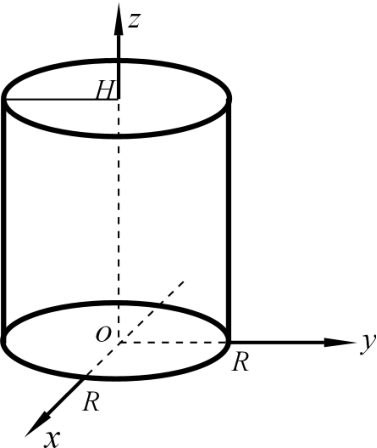
\includegraphics{./images/ch11/cg.pdf}}
\end{center}

{\bf 例:}\ps{同济}求球心在原点,半径为$R$的均质(密度$\mu$)对位于$(0,0,a)\;(a>R)$
处的单位质量的质点的引力。

[提示]:由对称性,显然$F_x=F_y=0$,
\begin{align*}
	F_z&=\iiint_{\Omega}G\mu\df{z-a}{[x^2+y^2+(z-a)^2]^{3/2}}\d V\\
	&=G\mu\dint_{-R}^R(z-a)\iint_{x^2+y^2\leq R^2-z^2}
	\df{1}{[x^2+y^2+(z-a)^2]^{3/2}}
	\d\sigma_{xy}\d z\\
	&=G\mu\dint_{-R}^R(z-a)
	\left(\df1{a-z}-\df1{\sqrt{R^2-2az+a^2}}\right)\d z\\
	&=-G\df M{a^2}
\end{align*}
其中$M=\df43\pi R^3\mu$为球的质量。

该结果表明:{\it 均质球对球外一质点的引力等于球的质量集中于球心时两质点间的引力。}

\subsection{空间曲面的表面积}

{\bf 例:}已知函数$z=f(x,y)\;(x,y)\in D$,求其对应曲面的表面积。

[分析]:在空间曲面$\Sigma:z=f(x,y)\;(x,y)\in D$上任一点$(x,y,f(x,y))$
处取面积微元$\d S$,设该微元在$xOy$平面上的投影为$\d\sigma_{xy}$,则
$$\d\sigma_{xy}=|\cos\gamma|\d S,$$
其中$\gamma$为$\d S$的法向量关于$z$轴的方向角。注意到$\d S$处的法向量为
$$\bm{n}=(f'_x,f'_y,-1),$$
故
$$|\cos\theta|=\df1{\sqrt{1+(f\,'_x)^2+(f\,'_y)^2}},$$
综上,所求面积
$${S=\iint_D\sqrt{1+(f\,'_x)^2+(f\,'_y)^2}\d\sigma_{xy}}$$

{\bf 例:}求半径为$R$的球的表面积。

[解]:上半球可表示为
$$z=\sqrt{R^2-x^2-y^2},\;(x^2+y^2\leq R^2),$$
注意到
$$z'_x=-\df xz,\quad z'_y=-\df yz,$$
故
$$\d S=\sqrt{1+(z'_x)^2+(z'_y)^2}\d\sigma_{xy}=\df Rz\d\sigma_{xy},$$
于是所求球的表面积为
\begin{align*}
	S&=2\iint_{x^2-y^2\leq R^2}\df Rz\d\sigma_{xy}\\
	&=2\dint_0^{2\pi}\dint_0^R\df R{\sqrt{R^2-\rho^2}}\rho\d\rho\d\theta
	=4\pi R^2
\end{align*}

{\bf 注:}掌握了求曲面面积的方法,我们将可以进一步得到求曲面质量、转动惯量、质心和
万有引力的方法。这些恰好就是下一章所要学习的第一型曲面积分的基本思想。

\section{习题课}

\subsection{二重积分的计算}

{\bf 例:}计算下列二重积分
\begin{enumerate}[(1)]
  \setlength{\itemindent}{1cm}
  \item $\ds\iint_Dxye^{xy^2}\d\sigma,\,D=\{0\leq x\leq 1,0\leq
  y\leq 1\}$ 
  \item $\ds\iint_D\df 1{x+y}\d\sigma,\,D=\{0\leq x\leq 1,1\leq x+y\leq
  2\}$ 
  \item $\ds\iint_D|x^2+y^2-4|\d\sigma,\,D=\{x^2+y^2\leq 9\}$ 
  \item $\ds\iint_D(x+y)\mathrm{sgn}(x-y)\d\sigma,\,D=\{0\leq x\leq 1,0\leq
  y\leq 1\}$
\end{enumerate}

{\bf 例:}改变下列累次积分的次序
\begin{enumerate}[(1)]
  \setlength{\itemindent}{1cm}
  \item $\dint_0^1\dint_0^xf(x,y)\d
  y\d x+\dint_1^2\dint_0^{2-x}f(x,y)\d y\d x$
  \item $\dint_0^{2a}\dint_{\sqrt{2ax-x^2}}^{\sqrt{2ax}}
  f(x,y)\d y\d x,\;(a>0)$ 
  \item $\dint_0^{2\pi}\dint_0^{\sin x}f(x,y)\d y\d x$
\end{enumerate}

{\bf 例:}设$f(x)$在区间$[a,b]$连续且恒大于零,证明:
$$\dint_a^bf(x)\d x\dint_a^b\df{\d x}{f(x)}\geq (b-a)^2$$

{\bf 例:}利用二重积分的方法证明
$$\left[\dint_a^bf(x)g(x)\d x\right]^2\leq
\dint_a^bf\,^2(x)\d x\dint_a^bg^2(x)\d x$$

{\bf 例:}设$f(x)$在$[a,b]$上单调递增且恒为正,证明
$${\dint_0^1xf\,^2(x)\d x}{\dint_0^1f(x)\d x}\leq
{\dint_0^1f\,^2(x)\d x}{\dint_0^1xf(x)\d x}$$

\subsection{二重积分与坐标变换}

{\bf 例:}计算
$$\iint_{x^2+y^2\leq 1}\df{\d\sigma}{(x^2+y^2)^m}$$

{\bf 例:}设$f(x)$可微,$f(0)=0,\,f\,'(0)=1$,求
$$\lim\limits_{t\to 0^+}\df 1{\pi t^3}
\iint_{x^2+y^2\leq t^2}f\left(
\sqrt{x^2+y^2}\right)\d x\d y$$

{\bf 一般的积分坐标变换}

设$x=x(u,v),y=y(u,v)$为一一映射、一阶偏导连续且$\df{\p(x,y)}{\p(u,v)}\ne0$,则
$$\iint_Df(x,y)dxdy=\iint_D f(x,y)\left|\df{\p(x,y)}{\p(u,v)}\right|
\d u\d v$$

{\bf 注:}对于三重积分,有类似的公式成立!

{\bf 例:}通过适当的变量替换,将下列二重积分化为定积分 
\begin{enumerate}[(1)]
  \setlength{\itemindent}{1cm}
  \item $\ds\iint_{|x|+|y|\leq 1}f(x+y)\d\sigma$ 
  \item $\ds\iint_Df(xy)\d\sigma$,$D$由$xy=1,xy=2,y=x,y=4x,(x>0,y>0)$围成 
%   \item $\ds\iint_{x^2+y^2\leq 1} f(ax+by+c)\d\sigma,\;(a^2+b^2\ne 0)$
\end{enumerate}

{\bf 例:}设$a^2+b^2=1,\, D:x^2+y^2\leq 1$,证明
$$\iint_Df(ax+by)\d\sigma_{xy}=2\dint_{-1}^1f(u)\sqrt{1-u^2}\d u.$$

[提示]:令$u=ax+by,\;v=bx-ay$,则
$$x^2+y^2\leq 1\quad\Leftrightarrow\quad u^2+v^2\leq 1.$$
且
$$\left|\df{\p(x,y)}{\p(u,v)}\right|=1,$$
于是
\begin{align*}
	\iint_{x^2+y^2\leq 1}&f(ax+by)\d\sigma_{xy}
	=\iint_{u^2+v^2\leq 1}f(u)\d\sigma_{uv}\\
	&=\dint_{-1}^1\dint_{-\sqrt{1-u^2}}^{\sqrt{1-u^2}}f(u)\d u
	=\dint_{-1}^1f(u)\sqrt{1-u^2}\d u
\end{align*}

\subsection{三重积分的计算}

{\bf 例:}设$f(z)$连续,证明:
$$\iiint_{x^2+y^2+z^2\leq 1}f(z)\d V=\pi\dint_{-1}^1f(u)(1-u^2)\d u$$

[提示]:使用“1+2”的方法。

{\bf 例:}计算积分
$$\iiint_{\Omega}(x+y+z)^2\d V,$$
其中$\Omega:\;\df{x^2}{a^2}+\df{y^2}{b^2}+\df{z^2}{c^2}\leq 1$

[提示]:注意到$\Omega$关于三个坐标面均对称,故
$$\iiint_{\Omega}xy\d V=\iiint_{\Omega}yz\d V=\iiint_{\Omega}zx\d V=0,$$
从而
$$\iiint_{\Omega}(x+y+z)^2\d V=\iiint_{\Omega}(x^2+y^2+z^2)\d V.$$

使用“1+2”计算积分,可得
$$\iiint_{\Omega}x^2\d V=\df4{15}\pi a^3bc,$$
注意到$\df xa,\df yb,\df zc$在$\Omega$内具有轮换对称性,故
$$\iiint_{\Omega}y^2\d V=\df4{15}\pi ab^3c,\quad
\iiint_{\Omega}z^2\d V=\df4{15}\pi abc^3.$$

综上,
$$\iiint_{\Omega}(x+y+z)^2\d V=\df4{15}\pi abc(a^2+b^2+c^2).$$


% {\bf 例:}计算三重积分
% $$\iiint_{\Omega}z^2\d V,\;\Omega:x^2+y^2+z^2\leq 1,\,z\geq 0$$

{\bf 例:}按给定的积分次序重写累次积分
$$\dint_0^1\dint_0^x\dint_0^{xy}f(x,y,z)\d z\d y\d x$$
\begin{enumerate}[(1)]
  \setlength{\itemindent}{1cm}
  \item 先$y$后$z$后$x$
  \item 先$x$后$z$后$y$
\end{enumerate}

\begin{center}
	\resizebox{!}{6cm}{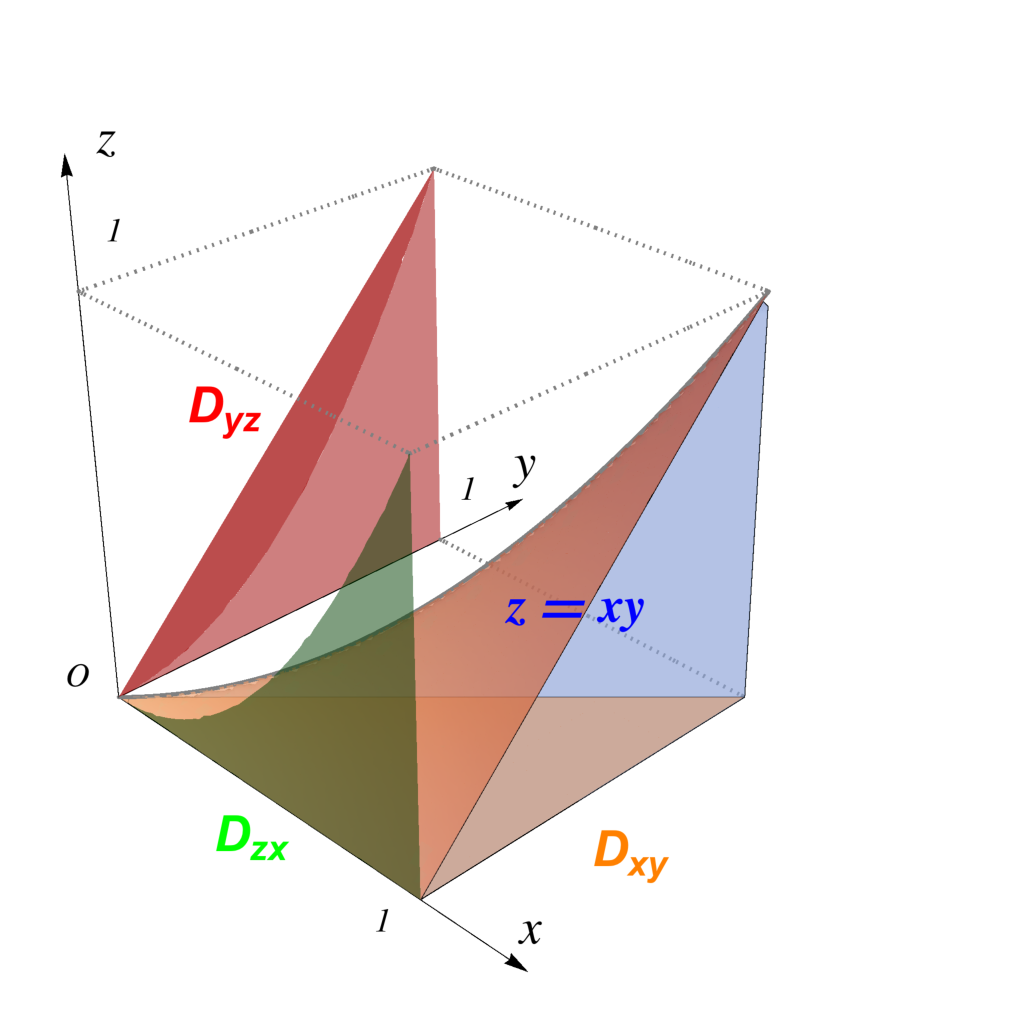
\includegraphics{./images/ch11/xyz2zxy.pdf}}
\end{center}

[提示](纯“代数”的定限方法)本例的积分区域可以描述为
$$\Omega:\;0\leq x\leq1,\;0\leq y\leq x,\;0\leq z\leq xy$$

(2)(先定$y$后定$z$再定$x$)首先考虑和$y$相关的不等式(对于包含$x,z$的部分,须
放缩至常数),有
$$0\leq y\leq x\leq 1,\quad 0\leq \df zx\leq y,$$
二者合并(取交集)可得$y$的变化范围
$$0\leq y\leq 1.$$

然后假设$y$给定,考虑和$z$相关的不等式(对于包含$x$的部分,须放缩至常数或与$y$有关的表示)
$$0\leq z\leq xy\leq y,$$
故$z$的变化范围为
$$0\leq z\leq y.$$

最后,与$x$相关的不等式包括:
$$y\leq x\leq 1,\quad \df zy\leq x,$$
注意到以$z=y^2$为分界线,以上两个不等式的左端大小关系可能反转,因此需要讨论。

最终定限结果为
$\Omega=\Omega_1+\Omega_2$,其中
$$\Omega_1:\;0\leq y\leq 1,\;0\leq z\leq y^2,\; y\leq x\leq 1,$$
$$\Omega_2:\;0\leq y\leq 1,\;y^2\leq z\leq 1,\; \df zy\leq x\leq 1.$$

{\bf 例:}求以下曲面在第一卦限中所围立体体积
$$\left(\df xa+\df yb\right)^2+\left(\df zc\right)^2=1,$$
其中$a,b,c>0$。

\begin{center}
	\resizebox{!}{6cm}{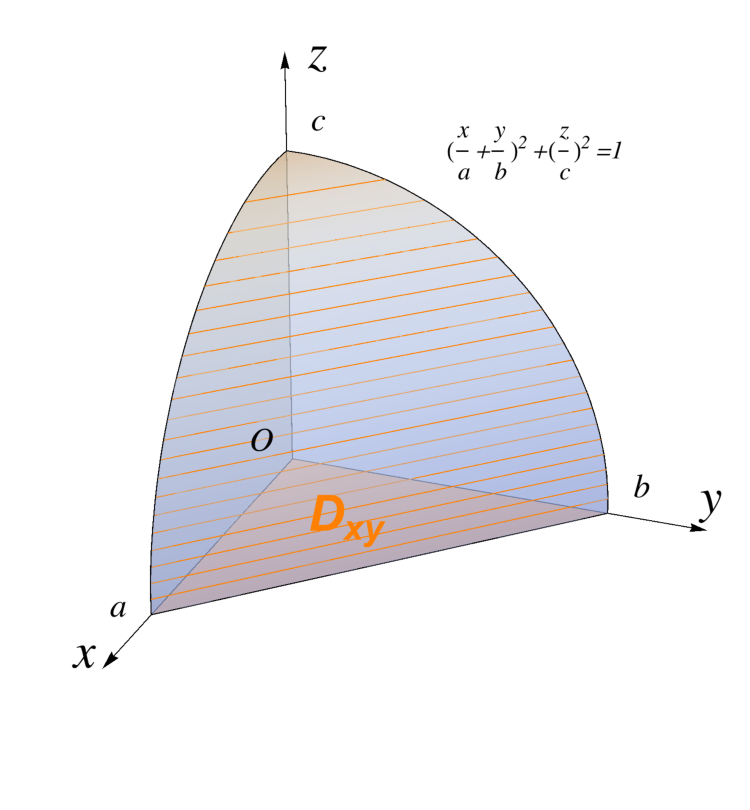
\includegraphics{./images/ch11/xy2z2.pdf}}
\end{center}

[提示]:\ps{本例的图形用手工方法很难描绘,故使用“代数”定限方法}积分区域可表示为
$$\Omega:\;\left(\df xa+\df yb\right)^2+\left(\df zc\right)^2\leq1,\;
x\geq0,\;y\geq0,\;z\geq0.$$

先定$z$。与之相关的不等式为
$$0\leq z\leq c\sqrt{1-\left(\df xa+\df yb\right)^2}\leq c,$$
故有$0\leq z\leq c$。

再定$(x,y)$。设$z$给定,则有
$$0\leq\df xa+\df yb\leq\sqrt{1-\left(\df zc\right)^2},
\;x\geq0,\;y\geq0,$$
对其定限可得
$$0\leq x\leq a\sqrt{1-\left(\df zc\right)^2},\;
0\leq y\leq b\left[\sqrt{1-\left(\df zc\right)^2}-\df xa\right],$$

至此,所求体积
$$V=\dint_0^c\dint_0^{a\sqrt{1-\left(\frac zc\right)^2}}
\dint_0^{b\left[\sqrt{1-\left(\frac zc\right)^2}-\frac xa\right]}
\d y\d x\d z=\df{abc}3.$$

\subsection{三重积分与坐标变换}

{\bf 例:}将三重积分
$$\dint_0^1\dint_{-\sqrt{y-y^2}}^{\sqrt{y-y^2}}
\dint_0^{\sqrt{3(x^2+3y^2)}}f\left(
\sqrt{x^2+y^2+z^2}\right)\d z\d x\d y$$
分别化为柱坐标和球坐标下的三重积分。

{\bf 例:}计算由以下平面所围成的立体体积:
$$a_ix+b_iy+c_iz=\pm h_i,\;i=1,2,3,$$
其中:$a_i,b_i,c_i(i=1,2,3)$为常数,且
$$\Delta=\left|\begin{array}{ccc}
a_1 & b_1 & c_1\\ a_2 & b_2 & c_2 \\ a_3 & b_3 & c_3
\end{array}\right|\ne 0$$

[提示]:设
$$u=a_1x+b_1y+c_1z,\;v=a_2x+b_2y+c_2z,\;w=a_3x+b_3y+c_3z,$$
则
$$\left|\df{\p(x,y,z)}{\p(u,v,w)}\right|=\df1{|\Delta|},$$
所求体积
$$V=\dint_{-|h_1|}^{|h_1|}\dint_{-|h_2|}^{|h_2|}\dint_{-|h_3|}^{|h_3|}
\df1{|\Delta|}\d w\d v\d u=\df{8|h_1h_2h_3|}{|\Delta|}.$$

{\bf 例:}计算极限
$$\lim\limits_{n\to\infty}\df 1{n^4}\iiint_{r\leq n}[r]\d V,$$
其中$r=\sqrt{x^2+y^2+z^2}$。

$${\df 43\pi\left[n^4-\sum\limits_{k=1}^nk^3\right]}$$

{\bf 例:}设$f(x)$可微,
$$F(t)=\iiint_{x^2+y^2+z^2\leq t^2}f(x^2+y^2+z^2)\d V,$$
求$F\,'(t)$。

% {\bf 例:}设$f(x)$可微,
% $$F(x)=\dint_0^x\d v\dint_0^v\d u\dint_0^uf(t)\d t,$$
% 求$F\,'(x)$。

\subsection{重积分的应用}

{\bf 例:}在一半径为$R$的球内,以某条直径为轴打一个高度为$2H(H<R)$的
圆孔,求打孔后球内剩余部分的体积。\ps{由此题可以得到一个有趣的结论:不论球的半径多大,
打孔后剩余的部分体积都是一样的!}

{\bf 例:}求锥面$3(x^2+y^2)=(z-3)^2$与$z=0$所围的内切球面
与该锥面所围成的立体的体积。

\subsection{$n$重积分*}

{\bf 例:}求$n$维单纯形
$$T_n:\; x_i\geq 0\,(i=1,2,\ldots,n),\;
\sum\limits_{i=1}^nx_i\leq a$$
的体积$(a>0)$。\ps{单纯形是三角形在高维空间中的推广}

[解]:定限\ps{使用纯“代数”的定限方法}
$$T_n:\;0\leq x_1\leq a,\;0\leq x_2\leq a-x_1,\;
0\leq x_3\leq a-x_1-x_2,$$
$$\ldots,\;0\leq x_n\leq a-x_1-x_2-\ldots-x_{n-1}$$
故所求体积
\begin{align*}
	V_n(a)&=\dint_0^a\dint_0^{a-x_1}\dint_0^{a-x_1-x_2}\ldots
	\dint_0^{a-x_1-x_2-\ldots-x_{n-1}}\d x_{n}\ldots\d x_3\d x_2\d x_1\\
	&=\dint_0^aV_{n-1}(a-x_1)\d x_1
\end{align*}
注意到
$$V_2(a)=\df12a^2,\quad V_3(a)=\df16a^3,$$
由数学归纳法,假设$V_{n-1}(a)=\df1{(n-1)!}a^{n-1}$,则
\begin{align*}
	V_n(a)&=\dint_0^aV_{n-1}(a-x_1)\d x_1\\
	&=\dint_0^a\df1{(n-1)!}(a-x_1)^{n-1}\d x_1=\df1{n!}a^n
\end{align*}
由此可知,假设成立,故
$$V_n(a)=\df1{n!}a^n.$$

用类似的方法可以证明:

{\bf 例:}证明:
$$\dint_0^t\d t_1\dint_0^{t_1}\d t_2\ldots
\dint_0^{t_{n-1}}\prod\limits_{i=1}^nf(t_i)\d t_n
=\df 1{n!}\left[\dint_0^tf(s)\d s\right]^n$$

{\bf 例:}求$n$维单位球
$$S_n:\;\sum\limits_{k=1}^nx_k^2\leq 1$$
的体积。

[解]:作$n$维球坐标变换
$$
\left\{\begin{array}{rl}
	x_1&=r\sin\theta_{n-1}\sin\theta_{n-2}\ldots\sin\theta_{2}\sin\theta_1\\
	x_2&=r\sin\theta_{n-1}\sin\theta_{n-2}\ldots\sin\theta_{2}\cos\theta_1\\
	x_3&=r\sin\theta_{n-1}\sin\theta_{n-2}\ldots\cos\theta_{2}\\
	\ldots&\ldots\\
	x_{n-1}&=r\sin\theta_{n-1}\cos\theta_{n-2}\\
	x_n&=r\cos\theta_{n-1}
\end{array}\right.
$$
对应的Jacobi行列式取绝对值后可表示为
$$\left|\df{\p(x_1,x_2,\ldots,x_n)}{\p(r,\theta_1,\ldots,\theta_{n-1})}\right|
=r^{n-1}J(\theta_1,\theta_2,\ldots,\theta_{n-1})$$
在球坐标系下,$S_n$可表示为
$$S_n:
\;(\theta_1,\theta_2,\ldots,\theta_{n-1})\in\Sigma_{n-1},
\;0\leq r\leq 1,$$
于是
\begin{align*}
	V_n&=\dint_{S_n}\d V_n\\
	&=\int\ldots\int_{\Sigma_{n-1}}\dint_0^1
	r^{n-1}\d rJ(\theta_1,\theta_2,\ldots,\theta_{n-1})
	\d\theta_{n-1}\ldots\d\theta_1\\
	&=\df1n\int\ldots\int_{\Sigma_{n-1}}
	J(\theta_1,\theta_2,\ldots,\theta_{n-1})\d\theta_{n-1}\ldots\d\theta_1
	=\df1nI_{n-1}
\end{align*}

以下来计算$I_{n-1}$。

\begin{align*}
	\pi^{n/2}&=\left(\dint_{-\infty}^{+\infty}e^{-x^2}\d x\right)^n\\
	&=\dint_{-\infty}^{+\infty}\dint_{-\infty}^{+\infty}\ldots
	\dint_{-\infty}^{+\infty}e^{-(x_1^2+x_2^2+\ldots+x_n^2)}\d x_n\ldots
	\d x_2\d x_1\\
	&=\int\ldots\int_{\Sigma_{n-1}}\dint_0^{+\infty}
	e^{-r^2}r^{n-1}J(\theta_1,\theta_2,\ldots,\theta_{n-1})
	\d r\d\theta_{n-1}\ldots\d\theta_1\\
	&=I_{n-1}\dint_0^{+\infty}e^{-r^2}r^{n-1}\d r
	=\df12I_{n-1}\dint_0^{+\infty}e^{-r^2}(r^2)^{n/2-1}\d r^2\\
	&=\df12I_{n-1}\dint_0^{+\infty}x^{n/2-1}e^{-x}\d x
	=\df12I_{n-1}\Gamma(n/2)
\end{align*}
从而
$$I_{n-1}=\df{2\pi^{n/2}}{\Gamma(n/2)},$$
进而可得
$$V_n=\df{2\pi^{n/2}}{n\Gamma(n/2)}.$$

{\bf 注:}注意到$\Gamma(n)=(n-1)!$,从以上的结果可以看到,随着维度的增加,
每增加一维,分子增大约$\sqrt{n}$倍,而分子固定地增大$\sqrt{\pi}$倍,这意味着$V_n$
是随着$n$的增大而不断递减的,且递减的速率越来越大。因此,可以很容易地得到如下的结论
$$\limn V_n=0.$$
换句话说,$n$维球的维度越高,则体积越小,并最终趋于零!

\section{小结}

这是充满“技术”的一章,而不是很偏重理论的一章,重点是掌握各种计算二重、三重积分的方法,
正确地加以运用。

本质上,重积分与定积分在概念上没有什么不同,都遵从“分割取近似,做和求极限”的思想来构造,
所不同的是,在计算的过程中,需要巧妙地将重积分分解成一系列相互嵌套的定积分,而这种分解
成功的关键,是正确给定每个积分变量的积分区间,或者说,定限。

定限,从技术上说,存在两种看起来截然不同的思路,一种依赖于对图形的分析,这时能够正确地
作图就显得很重要了,另一种则几乎是纯“代数”的,从已知的不等式出发,逐步分解(分析)出每个变量
的变化范围,这种情况下,正确描述出各变量变化范围的依存关系既是解题的关键,也是难点。

至于积分的计算,是一个容易被忽视,却常常成为无法求得结果的主要障碍的问题。从这个意义上
说,重积分计算的技术很大程度上还是要依赖于对定积分的掌握,事实上,本学期大多数的章节都
可以看到一元函数微积分的影子,这一点对于我们更深入地理解整个高等数学的知识体系其实也是
至关重要的。

接下来,进入曲线和曲面积分前,请不要忘记以上的思想,它会是我们真正克服各种理解障碍的有力
工具。

\newpage

\section*{课后作业}
\addcontentsline{toc}{section}{课后作业}

{\bf 【必作题】}

\begin{itemize}
  \setlength{\itemindent}{1cm}
  \item 习题11.1:7,10
  \item 习题11.2:1(3,4),4(2,3),5,6(2),7(1),9,11,13(1),15(2),17,19,24
  \item 习题11.3:3(3),7(3,4),8(2),10,11(3,4),12,13,14,16,19
  \item 习题11.4:2,4,7,8,12,14,15
\end{itemize}

\bigskip

\hrule

\bigskip

{\bf 【思考题】}

1、改变下列累次积分的次序\ps{常见考点}
\begin{enumerate}[(1)]
  \setlength{\itemindent}{1cm}
  \item $\dint_0^{2a}\dint_{\sqrt{2ax-x^2}}^{\sqrt{2ax}}
  f(x,y)\d y\d x,\;(a>0)$ 
  \item $\dint_0^{2\pi}\dint_0^{\sin x}f(x,y)\d y\d x$
\end{enumerate}

2、设$f(x)$在$[a,b]$上单调递增且恒非负,证明\ps{参考Cauchy-Schwarz不等式的证明}
$${\dint_a^b xf\,^2(x)\d x}{\dint_a^b f(x)\d x}\geq
{\dint_a^b f\,^2(x)\d x}{\dint_a^b xf(x)\d x}$$

3、设$f(x)$可微,$f(0)=0,\,f\,'(0)=1$,求\ps{常考的类型}
$\lim\limits_{t\to 0^+}\df 1{\pi t^3}
\iint_{x^2+y^2\leq t^2}f\left(
\sqrt{x^2+y^2}\right)\d x\d y$

4、计算二重积分$\ds\iint_D xy\d\sigma$,其中$D$由$xy=1,xy=2,y=x,y=4x$围成。
\ps{利用一般的坐标变换计算重积分} 

5、设$f(z)$连续,证明:\ps{常见类型}
$$\iiint_{x^2+y^2+z^2\leq 1}f(z)\d V=\pi\dint_{-1}^1f(u)(1-u^2)\d u$$

6、按先$x$后$z$后$y$的积分次序重写累次积分\ps{三重积分定限练手的好题目}
$$\dint_0^1\dint_0^x\dint_0^{xy}f(x,y,z)\d z\d y\d x$$

7、计算积分\ps{注意对称性的应用!}
$$\iiint_{\Omega}(x+y+z)^2\d V,$$
其中$\Omega:\;\df{x^2}{a^2}+\df{y^2}{b^2}+\df{z^2}{c^2}\leq 1$。
% \quad{\it (提示:由对称性,原式$=\ds\iiint_{\Omega}(x^2+y^2+z^2)\d V$)}

8、计算由以下平面所围成的立体体积:\ps{利用一般的坐标变换计算重积分,相对于纯的几何方法
——参见第八章——可展示出极大的简便性!}
$$a_ix+b_iy+c_iz=\pm h_i,\;i=1,2,3,$$
其中:$a_i,b_i,c_i(i=1,2,3)$为常数,且
$$\Delta=\left|\begin{array}{ccc}
a_1 & b_1 & c_1\\ a_2 & b_2 & c_2 \\ a_3 & b_3 & c_3
\end{array}\right|\ne 0$$

9、求$n$维单纯形$T_n:\; x_i\geq 0\,(i=1,2,\ldots,n),\;
\sum\limits_{i=1}^nx_i\leq a$
的体积$(a>0)$。\ps{检验对纯代数的定限方法的掌握}

10、证明:
$$\dint_0^t\d t_1\dint_0^{t_1}\d t_2\ldots
\dint_0^{t_{n-1}}\prod\limits_{i=1}^nf(t_i)\d t_n
=\df 1{n!}\left[\dint_0^tf(s)\d s\right]^n$$

% \visibletrue
\ifvisible

\newpage

\section*{关于$n$重积分}
\addcontentsline{toc}{section}{关于$n$重积分}

{\bf 例:}求$n$维单位球的体积。

{\bf 解:}令
$$
\left\{
\begin{array}{l}
x_1=r\sin\theta_1\sin\theta_2\cdots\sin\theta_{n-2}\sin\theta_{n-1}\\
x_2=r\sin\theta_1\sin\theta_2\cdots\sin\theta_{n-2}\cos\theta_{n-1}\\
x_3=r\sin\theta_1\sin\theta_2\cdots\cos\theta_{n-2}\\
\cdots\hspace{1cm}\cdots\hspace{1cm}\cdots\\
x_{n-1}=r\sin\theta_1\cos\theta_2\\
x_n=r\cos\theta_1
\end{array}
\right..
$$
则$n$维单位球$S_n:\sum\limits_{i=1}^nx^2_i\leq1$可表示为
$$0\leq r\leq 1,\;(\theta_1,\theta_2,\ldots,\theta_{n-1})\in\Sigma_{n-1}.$$
又
$$J=\df{\p(x_1,x_2,\ldots,x_n)}{\p(r,\theta_1,\ldots,\theta_{n-1})}
=r^{n-1}\Delta_{n-1},$$
其中$\Delta_{n-1}$为某个关于$(\theta_1,\theta_2,\ldots,\theta_{n-1})$的函数,记
$$I_{n-1}=\dint\ldots\dint_{\Sigma_{n-1}}|\Delta_{n-1}|
\d\theta_1\ldots\d\theta_{n-1},$$
于是
$n$维单位球的体积
$$V_n=\dint\ldots\dint_{\Omega_n}\d V
=\dint_0^1\left[\dint\ldots\dint_{\Sigma_{n-1}}r^{n-1}|\Delta_{n-1}|
\d\theta_1\ldots\d\theta_{n-1}\right]\d r=\df1nI_{n-1}.$$

以下求$I_{n-1}$。注意到
$$\pi^{\frac n2}=\left(\dint_{-\infty}^{+\infty}e^{-x^2}\d x\right)^n
=\dint\ldots\dint_{\mathbb{R}^n}e^{-(x_1^2+\ldots+x_n^2)}\d V,$$
使用前述变换,$\mathbb{R}^n$可表示为
$$0\leq r<+\infty,
\;(\theta_1,\theta_2,\ldots,\theta_{n-1})\in\Sigma_{n-1}.$$
从而(注:$\Gamma(s)=\dint_0^{+\infty}e^{-x}x^{s-1}\d x$)
\begin{eqnarray*}
	\pi^{\frac n2}&=&\dint_0^{+\infty}
	\left[\dint\ldots\dint_{\Sigma_{n-1}}e^{-r^2}r^{n-1}|\Delta_{n-1}|
	\d\theta_1\ldots\ldots\d\theta_{n-1}\right]\d r\\
	&=&I_{n-1}\dint_0^{+\infty}e^{-r^2}r^{n-1}\d r
	=I_{n-1}\df{\Gamma\left(\df{n}2\right)}2.
\end{eqnarray*}
故
$$I_{n-1}=\df{2\pi^{\frac n2}}{\Gamma\left(\df{n}2\right)},$$
进而可得
$$V_n=\df{2\pi^{\frac n2}}{n\Gamma\left(\df{n}2\right)}.$$

{\bf 推论:}$\limn V_n=0$.

{\bf 证明:}注意到$\Gamma(s)=(s-1)\Gamma(s-1)$,取$N=[8\pi]+1$,则对$\forall n>N$有
$$\df{V_{n+2}}{V_n}=\df{2\pi(n+2)}{n^2}<\df12.$$
于是
$$0<V_n<\left(\df12\right)^{\left[\frac{n-N}2\right]}V_N,$$
显然$\left(\df12\right)^{\left[\frac{n-N}2\right]}V_N\to0(n\to\infty)$,利用夹逼定理,
即证。

% \fi

\newpage

\begin{center}
	{\Large\bf 选择题测试}
	
	{\it (60分钟,每题3分,总分:99+1)}
\end{center}

\begin{enumerate}
  \item 设$x,e^x,e^{2x}$分别为方程$y''+p(x)y'+q(x)y=f(x)$的三个解,则
  该方程满足$y(0)=1,y'(0)=3$的特解为
  (\underline{\hspace{1cm}})
  %\ps{A}
  
  (A)$2e^{2x}-e^x$\hspace{1cm}(B)$e^x-2e^{2x}$ \hspace{1cm}
  (C)$e^{2x}-e^x$\hspace{1cm}(D)$2e^{2x}-\cos x$
%   \begin{enumerate}[(A)]
%     \item $2e^{2x}-e^x$
%     \item $e^x-2e^{2x}$
%     \item $e^{2x}-e^x$
%     \item $2e^{2x}-\cos x$
%   \end{enumerate}
  \item 方程$y''+y=x^2+1+\sin x$的特解可设为
  (\underline{\hspace{1cm}})
  %\ps{C}
  \begin{enumerate}[(A)]
    \item $y^*=ax^2+bx+c+x(A\sin x+B\cos x)$
    \item $y^*=x(ax^2+bx+c+A\sin x+B\cos x)$
    \item $y^*=ax^2+bx+c+A\sin x$
    \item $y^*=ax^2+bx+c+A\cos x$
  \end{enumerate}
  \item 二重极限$\lim\limits_{(x,y)\to(0,0)}\df{xy^2}{x^2+y^4}=$
  (\underline{\hspace{1cm}})
  %\ps{D}  
  
  (A) $0$\hspace{1cm}(B) $1$  \hspace{1cm}(C)$\df12$\hspace{1cm}(D)不存在
  \item 函数$f(x,y)=x^2-ay^2$($a$为常数)在$(0,0)$处(\underline{\hspace{1cm}})
  %\ps{D}
  
  (A) 不取极值\quad(B)取极小值\quad (C)取极大值\quad
  (D)是否取极值取决于$a$的值
%   \begin{enumerate}[(A)]
%     \item 不取极值
%     \item 取极小值
%     \item 取极大值
%     \item 是否取极值取决于$a$的值
%   \end{enumerate}
  \item 函数$f(x,y)=\left\{\begin{array}{ll}
  0&,(x,y)=(0,0)\\
  \df{xy}{x^2+y^2}&,else
  \end{array}\right.$在原点处(\underline{\hspace{1cm}})
  %\ps{B}
  \begin{enumerate}[(A)]
    \item 连续且存在偏导数
    \item 不连续但存在偏导数
    \item 连续但不存在偏导数
    \item 不连续也不存在偏导数
  \end{enumerate}
  \item 函数$z=\sqrt{x^2+y^2}$在原点处 
  (\underline{\hspace{1cm}})
  %\ps{C}
  \begin{enumerate}[(A)]
    \item 偏导数和各方向的方向导数均存在
    \item 偏导数不存在,但各方向的方向导数均存在
    \item 偏导数和各方向的方向导数均不存在
    \item 偏导数存在,但某些方向的方向导数不存在
  \end{enumerate}
  \item 曲面$z=x+f(x-z)$的所有切平面都与某定直线
  (\underline{\hspace{1cm}})
  %\ps{B}
  
  (A) 垂直\hspace{1cm}(B) 平行  \hspace{1cm}(C)夹角为$\pi/4$\hspace{1cm}
  (D)夹角为$\pi/3$
%   \begin{enumerate}[(A)]
%     \item 垂直
%     \item 平行
%     \item 夹角为$\pi/4$
%     \item 夹角为$\pi/3$
%   \end{enumerate}
  \item 设$f(x,y)=(y-x^2)(y-x^4)$,$P(0,0),M(1,1)$,则(\underline{\hspace{1cm}})
%   \ps{B}
  \begin{enumerate}[(A)]
    \item $P,M$均为$f(x,y)$的极值点
    \item $P,M$均不是$f(x,y)$的极值点
    \item $P$为$f(x,y)$的极值点,$M$不是
    \item $M$为$f(x,y)$的极值点,$P$不是
  \end{enumerate}
  \item $x^2+y^2=1$时,$f(x,y)=(x^2+y^2)e^{-(x^2+y^2)}$ 
  (\underline{\hspace{1cm}})
%   \ps{B}
  
  (A)不取极值\hspace{1cm}(B)取极大值 \hspace{1cm}
  (C)取极小值\hspace{1cm}(D)取最大值
%   \begin{enumerate}[(A)]
%     \item 不取极值
%     \item 取极大值
%     \item 取极小值
%     \item 取最大值
%   \end{enumerate}
  \item $f(x,y)$在原点附近连续,$\lim\limits_{(x,y)\to(0,0)}
  \df{f(x,y)-|xy|}{(x^2+y^2)^2}=1$,则$f(x,y)$在原点
  (\underline{\hspace{1cm}})
%   \ps{C}
  
  (A)不取极值\hspace{1cm}(B)取极大值 \hspace{1cm}(C)取极小值\hspace{1cm}
  (D)不一定取极值
%   \begin{enumerate}[(A)]
%     \item 不取极值
%     \item 取极大值
%     \item 取极小值
%     \item 不一定取极值
%   \end{enumerate}
  \item $D$是顶点为$(1,0),(1,1),(2,0)$的三角区域,
  $I_k=\ds\iint_D[\ln(x+y)]^k\d\sigma$,则(\underline{\hspace{1cm}})
%   \ps{B}
  
  (A)$I_1<I_2<I_3$\quad(B)$I_1>I_2>I_3$\quad
  (C)$I_1<I_3<I_2$\quad(D)$I_3<I_1<I_2$
%   \begin{enumerate}[(A)]
%     \item $I_1<I_2<I_3$
%     \item $I_1>I_2>I_3$
%     \item $I_1<I_3<I_2$
%     \item $I_3<I_1<I_2$
%   \end{enumerate}
  \item 设$D_1:x+y\leq1,x\geq 0,y\geq0;\,D_2:|x|+|y|\leq1$,
  $I_j=\ds\iint_{D_j}e^{|x|+|y|}\d\sigma(j=1,2)$,则
  (\underline{\hspace{1cm}})
%   \ps{C}
  
  (A)$I_1=I_2$\hspace{1cm}(B)$2I_1=I_2$\hspace{1cm}
  (C)$4I_1=I_2$\hspace{1cm}(D)$I_1=4I_2$
%   \begin{enumerate}[(A)]
%     \item $I_1=I_2$
%     \item $2I_1=I_2$
%     \item $4I_1=I_2$
%     \item $I_1=4I_2$
%   \end{enumerate}
  \item 设$\ds\iint_{x^2+y^2\leq a^2}\sqrt{a^2-x^2-y^2}\d\sigma=\pi$,
  则$a=$(\underline{\hspace{1cm}})
%   \ps{D}
  
  (A)$1$\hspace{1cm}(B)$\sqrt[3]{\df12}$\hspace{1cm}
  (C)$\sqrt[3]{\df34}$\hspace{1cm}(D)$\sqrt[3]{\df32}$
%   \begin{enumerate}[(A)]
%     \item $1$
%     \item $\sqrt[3]{\df12}$
%     \item $\sqrt[3]{\df34}$
%     \item $\sqrt[3]{\df32}$
%   \end{enumerate}
  \item 设$\Omega$为$z\geq{\sqrt{x^2+y^2}}(z\geq0)$介于$z=1$和$z=2$之间
  的部分,则$\ds\iiint_{\Omega}f(x^2+y^2+z^2)\d V=$
  (\underline{\hspace{1cm}})
%   \ps{A}
  \begin{enumerate}[(A)]
    \item $\dint_1^2\dint_0^{2\pi}\dint_0^zf(r^2+z^2)r\d r\d\theta\d z$
    \item $\dint_0^{2\pi}\dint_1^2r\dint_0^1f(r^2+z^2)\d z\d r\d\theta$
    \item $\dint_0^{2\pi}\dint_0^{\frac{\pi}4}\dint_1^2
    f(r^2)r^2\sin\varphi\d r\d\varphi\d\theta$
    \item $\dint_0^{2\pi}\dint_{\frac{\pi}2}^{\frac{\pi}4}\dint_1^2
    f(r^2)r^2\sin\varphi\d r\d\varphi\d\theta$
  \end{enumerate}
  \item 设$\Gamma$为上半圆周$x^2+y^2=2x$从原点到$(1,1)$的部分,则
  $\dint_{\Gamma}P(x,y)\d x+Q(x,y)\d y=$(\underline{\hspace{1cm}})
%   \ps{C}
  \begin{enumerate}[(A)]
    \item $\dint_{\Gamma}\left[P(x,y)(x-1)+Q(x,y)\sqrt{2x-x^2}\right]\d s$
    \item $\dint_{\Gamma}\left[P(x,y)(1-x)-Q(x,y)\sqrt{2x-x^2}\right]\d s$
    \item $\dint_{\Gamma}\left[P(x,y)\sqrt{2x-x^2}+Q(x,y)(1-x)\right]\d s$
    \item $\dint_{\Gamma}\left[-P(x,y)\sqrt{2x-x^2}+Q(x,y)(x-1)\right]\d s$
  \end{enumerate}
  \item 设$f(x)$可微,$f(0)=1$,则$\lim\limits_{t\to0^+}\df1{\pi t^3}
  \ds\iint_{x^2+y^2\leq t^2}  f(\sqrt{x^2+y^2})\d x\d y=$ 
  (\underline{\hspace{1cm}})
%   \ps{C}
  
  (A)$0$\hspace{1cm}(B)$\df23f'(0)$\hspace{1cm}
  (C)$+\infty$\hspace{1cm}(D)不存在但也不是$\infty$
%   \begin{enumerate}[(A)]
%     \item $0$
%     \item $\df23f'(0)$
%     \item $+\infty$
%     \item 不存在但也不是$\infty$
%   \end{enumerate}
  \item 设$\Gamma$为$A(-1,0),B(-3,2)$和$C(3,0)$为顶点的三角形区域沿$ABCA$方向
  的封闭折线,则$\ds\oint_{\Gamma}(3x-y)\d x+(x-2y)\d y=$
  (\underline{\hspace{1cm}})
%   \ps{D}
  
  (A)$16$\hspace{1cm}(B)$-16$\hspace{1cm}
  (C)$8$\hspace{1cm}(D)$-8$
%   \begin{enumerate}[(A)]
%     \item $16$
%     \item $-16$
%     \item $8$
%     \item $-8$
%   \end{enumerate}
  \item 设$S$为单位球的外侧,$S_1$为其上半部分,则下列等式成立的是
  (\underline{\hspace{1cm}})
%   \ps{A}
  \begin{enumerate}[(A)]
    \item $\ds\iint_{S}|z|\d S=2\ds\iint_{S_1}|z|\d S$
    \item $\ds\iint_{S}|z|\d x\d y=2\ds\iint_{S_1}|z|\d x\d y$
    \item $\ds\iint_{S}|y|\d x\d y=2\ds\iint_{S_1}|y|\d x\d y$
    \item $\ds\iint_{S}|x|\d x\d y=2\ds\iint_{S_1}|x|\d x\d y$
  \end{enumerate}
  \item 设$S$为$z=\sqrt{x^2+y^2}$被$z=1$所截得的有限部分的外侧,则
  $\ds\iint_S x\d y\d z+y\d z\d x+(z^2-2z)\d x\d y=$
  (\underline{\hspace{1cm}})
%   \ps{D}
  
  (A)$-\df32\pi$\hspace{1cm}(B)$0$\hspace{1cm}
  (C)$\df{\pi}2$\hspace{1cm}(D)$\df32\pi$
%   \begin{enumerate}[(A)]
%     \item $-\df32\pi$
%     \item $0$
%     \item $\df{\pi}2$
%     \item $\df32\pi$
%   \end{enumerate}
  \item 设$L_1:\df{x^2}{4}+\df{y^2}{9}=1,L_2:\df{x^2}{9}+\df{y^2}{4}=1$,
  二者所围封闭区域分别为$D_1,D_2$,则下列正确的是
  (\underline{\hspace{1cm}})
%   \ps{C}
  \begin{enumerate}[(A)]
    \item $\dint_{L_1}(x+y^2)\d s=2\dint_{L_2}y^2\d s$
    \item $\dint_{L_1}(x^2+y)\d s=2\dint_{L_2}(x^2+y)\d s$
    \item $\ds\iint_{D_1}(x+y^3)\d\sigma=2\ds\iint_{D_2}(x+y^3)\d\sigma$
    \item $\ds\iint_{D_1}(x^2+y)\d\sigma=2\ds\iint_{D_2}(x^2+y)\d\sigma$
  \end{enumerate}
  \item $f(x,y)$偏导连续,曲线$L:f(x,y)=1$过第二象限的点$M$
  和第四象限的点$N$,$\Gamma$为$L$上从$M$到$N$的一段弧,则下列
  小于零的是
  (\underline{\hspace{1cm}})
%   \ps{B}
  \begin{enumerate}[(A)]
    \item $\dint_{\Gamma}f(x,y)\d x$
    \item $\dint_{\Gamma}f(x,y)\d y$
    \item $\ds\int_{\Gamma}f(x,y)\d s$
    \item $\ds\int_{\Gamma}f\,'_x(x,y)\d x+f\,'_y(x,y)\d y$
  \end{enumerate}
  \item 设曲面$S_1:x^2+y^2+z^2=1(z\geq
  0)$,$S_2$为$S_1$在第一卦限中的部分,
  则以下正确的是
  (\underline{\hspace{1cm}})
%   \ps{C}
  \begin{enumerate}[(A)]
    \item $\ds\iint_{S_1}x\d S=4\iint_{S_2}x\d S$
    \item $\ds\iint_{S_1}y\d S=4\iint_{S_2}x\d S$
    \item $\ds\iint_{S_1}z\d S=4\iint_{S_2}x\d S$
    \item $\ds\iint_{S_1}xyz\d S=4\iint_{S_2}xyz\d S$
  \end{enumerate}
  \item 设$f(r)$二阶连续可微,$r=\sqrt{x^2+y^2+z^2}$,
  若$\mathrm{div}(\bigtriangledown\,f(r))=0$,则$f(r)=$
  (\underline{\hspace{1cm}})
%   \ps{B}
  
  (A)$C_1r+C_2$\hspace{1cm}(B)$C_1/r+C_2$\hspace{1cm}
  (C)$C_1r^2+C_2$\hspace{1cm}(D)$C_1/r^2+C_2$
%   \begin{enumerate}[(A)]
%     \item $C_1r+C_2$
%     \item $C_1/r+C_2$
%     \item $C_1r^2+C_2$
%     \item $C_1/r^2+C_2$
%   \end{enumerate}
  以上$C_1,C_2$为任意常数
  \item 设$\Gamma$是从原点沿折线$y=1-|x-1|$至点$(2,0)$,则
  $\dint_{\Gamma}-y\d x+x\d y=$
  (\underline{\hspace{1cm}})
%   \ps{D}
  
  (A)$0$\hspace{1cm}(B)$-1$\hspace{1cm}
  (C)$2$\hspace{1cm}(D)$-2$
%   \begin{enumerate}[(A)]
%     \item 0
%     \item -1
%     \item 2
%     \item -2
%   \end{enumerate}
  \item 设$S$是三个坐标面与平面$x=a,y=b,z=c$(其中$a,b,c$均大于零)所围成的
  封闭曲面的外侧,则$\ds\oiint_S(x^2-yz)\d y\d z+(y^2-zx)\d z\d x
  +(z^2-xy)\d x\d y=$
  (\underline{\hspace{1cm}})
%   \ps{A}
  \begin{enumerate}[(A)]
    \item $abc(a+b+c)$
    \item $a^2b^2c^2(a+b+c)$
    \item $ab+ac+bc$
    \item $(a+b+c)^2$
  \end{enumerate}
  \item 若$(x^4+4xy^3)\d x+(ax^2y^2-5y^4)\d y$为全微分,则其原函数为
  (\underline{\hspace{1cm}})
%   \ps{C}
  \begin{enumerate}[(A)]
    \item $\df15x^5+3x^2y^2-y^5+C$
    \item $\df15x^5+4x^2y^2-5y^4+C$
    \item $\df15x^5+2x^2y^3-y^5+C$
    \item $\df15x^5+2x^2y^3-5y^4+C$
  \end{enumerate}
  \item 设$\sumn(-1)^n\df{(x-a)^n}n$在$x>0$时发散,在$x=0$处收敛,则$a=$
  (\underline{\hspace{1cm}})
%   \ps{B}
  
  (A)$1$\hspace{1cm}(B)$-1$\hspace{1cm}
  (C)$2$\hspace{1cm}(D)$-2$
%   \begin{enumerate}[(A)]
%     \item 1
%     \item -1
%     \item 2
%     \item -2
%   \end{enumerate}
  \item 设$\sumn a_n(x-1)^n$在$x=-1$处收敛,则它在$x=2$处
  (\underline{\hspace{1cm}})
%   \ps{B}
  
  (A)发散\hspace{1cm}(B)绝对收敛\hspace{1cm}
  (C)条件收敛\hspace{1cm}(D)敛散性与$a_n$有关
%   \begin{enumerate}[(A)]
%     \item 发散
%     \item 绝对收敛
%     \item 条件收敛
%     \item 敛散性与$a_n$有关
%   \end{enumerate}
  \item 设$\sumn a_nx^n$和$\sumn b_nx^n$收敛半径均为$R$,
  $\sumn(a_n+b_n)x^n$收敛半径为$R_1$,则
  (\underline{\hspace{1cm}})
%   \ps{C}
  
  (A)$R=R_1$\hspace{1cm}(B)$R>R_1$\hspace{1cm}
  (C)$R\leq R_1$\hspace{1cm}(D)$R\geq R_1$
  \item 若级数$\sumn a_n$条件收敛,则$\sumn na_n(x-1)^n$在$x=\sqrt3$和$x=3$分别
  (\underline{\hspace{1cm}})
%   \ps{B}
  
  (A)收敛,收敛\hspace{1cm}(B)收敛,发散\hspace{1cm}
  (C)发散,收敛\hspace{1cm}(D)发散,发散
%   \begin{enumerate}[(A)]
%     \item $R=R_1$
%     \item $R>R_1$
%     \item $R\leq R_1$
%     \item $R\geq R_1$
%   \end{enumerate}
  \item 设$f(x)=\left\{\begin{array}{ll}
  x&,x\in[0,1/2]\\ 2(1-x)&,x\in(1/2,1)
  \end{array}\right.$,$S(x)=\df{a_0}2+\sumn a_n\cos n\pi x,
  (x\in\mathbb{R})$,其中$a_n=2\dint_0^1f(x)\cos n\pi x\d x
  (n=0,1,2,\ldots)$,则$S\left(-\df52\right)=$
  (\underline{\hspace{1cm}})
%   \ps{A}
  
  (A)$\df34$\hspace{1cm}(B)$\df12$\hspace{1cm}
  (C)$-\df34$\hspace{1cm}(D)$-\df12$
%   \begin{enumerate}[(A)]
%     \item $\df34$
%     \item $\df12$
%     \item $-\df34$
%     \item $-\df12$
%   \end{enumerate}
  \item 将函数$f(x)=\left\{\begin{array}{ll}
  1&,0\leq x<1\\ x+1&,1\leq x\leq \pi
  \end{array}\right.$在$[0,\pi]$上展开成余弦级数,则其和函数在$x=1$和$x=\pi$
  处的值分别为
  (\underline{\hspace{1cm}})
%   \ps{A}
  
  (A)$\df32,\pi+1$\hspace{1cm}(B) $2,0$\hspace{1cm}
  (C)$2,\pi+1$\hspace{1cm}(D)$\df32,\df{\pi}2+1$
%   \begin{enumerate}[(A)]
%     \item $\df32,\pi+1$
%     \item $2,0$
%     \item $2,\pi+1$
%     \item $\df32,\df{\pi}2+1$
%   \end{enumerate}
  \item 设$f(x)$连续,则$\dint_0^1\d y\dint_{-\sqrt{1-y^2}}^{1-y}f(x,y)\d y=$
  (\underline{\hspace{1cm}})
%   \ps{D}
  \begin{enumerate}[(A)]
    \item $\dint_0^1\d x\dint_{0}^{x-1}f(x,y)\d y
    +\dint_{-1}^0\d x\dint_0^{\sqrt{1-x^2}}f(x,y)\d y$
    \item $\dint_0^1\d x\dint_{0}^{1-x}f(x,y)\d y
    +\dint_{-1}^0\d x\dint_{-\sqrt{1-x^2}}^0f(x,y)\d y$
    \item $\dint_0^{\frac{\pi}2}\d\theta\dint_0^{\frac1{\cos\theta+\sin\theta}}
    f(r\cos\theta,r\sin\theta)\d r+\dint_{\frac{\pi}2}^{\pi}\d\theta
    \dint_0^1f(r\cos\theta,r\sin\theta)\d r$
    \item $\dint_0^{\frac{\pi}2}\d\theta\dint_0^{\frac1{\cos\theta+\sin\theta}}
    f(r\cos\theta,r\sin\theta)r\d r+\dint_{\frac{\pi}2}^{\pi}\d\theta
    \dint_0^1f(r\cos\theta,r\sin\theta)r\d r$
  \end{enumerate}
  
\end{enumerate}

% \ifvisible

\newpage

{\Large\bf 第11章习题课作业}

{\it (请抄题)}

1、交换积分次序
 \begin{enumerate}[(1)]
    \setlength{\itemindent}{1cm}
    \item $\dint_0^2\dint_{x^2}^xf(x,y)\d y\d x$
    \item $\dint_{-\pi/4}^{\pi/2}\dint_0^{2a\cos\theta}
    f(\rho\cos\theta,\rho\sin\theta)\rho\d\rho\d\theta$
 \end{enumerate}
 
2、设$f(x)$在$[a,b]$上单调递增且恒为正,证明
	$${\dint_0^1xf\,^2(x)\d x}{\dint_0^1f(x)\d x}\leq
	{\dint_0^1f\,^2(x)\d x}{\dint_0^1xf(x)\d x}$$

[提示:参考Cauchy-Schwarz积分不等式的证明方法]
	
3、计算极限
	$\lim\limits_{n\to\infty}\df 1{n^4}\iiint_{r\leq n}[r]\d V,$
	其中$r=\sqrt{x^2+y^2+z^2}$
	
4、$f(t)$连续,$F(t)=\ds\iiint_{\Omega}[z^2+f(x^2+y^2)]\d V$,其中
	$\Omega$由$x^2+y^2\leq t^2,0\leq z\leq h$确定,求$F'(t)$和
	$\lim\limits_{t\to 0^+}\df{F(t)}{t^2}$

5、求由四条直线$x+y=p,x+y=q,y=ax,y=bx$,其中$0<p<q,0<a<b$所围平面图形的面积。

6、计算三重积分$\ds\iiint_{\Omega}(x+y)\d V$,其中$\Omega$由
$x=0,x=1,x^2+1=\df{y^2}{b^2}+\df{z^2}{c^2}$所围成。

[提示:注意使用对称性!]

7、设$\Omega:z\geq x^2+y^2,z\leq x$,将积分
$\ds\iiint_{\Omega}f(x,y,z)\d V$分别化成柱坐标和球坐标下的累次积分。

% 8(选作)、求$\ds\iiint_{\Omega}\df{\d V}r$,其中$\Omega$为任一
% 半径为$R$的球,$r$为球外一固定点到球内任一点的距离。
% 
% [提示:不妨设固定点为原点,球心坐标为$(x_0,y_0,z_0)$,作带有平移的球坐标变换
% $$\left\{\begin{array}{l}
% x=x_0+r\sin\varphi\cos\theta,\\
% y=y_0+r\sin\varphi\sin\theta,\\
% z=z_0+r\cos\varphi
% \end{array}\right.$$
% ]

8(选作)、设$a^2+b^2=1,\, D:x^2+y^2\leq 1$,证明
$$\iint_Df(ax+by)\d x\d y=2\dint_{-1}^1f(u)\sqrt{1-u^2}\d u.$$

[提示:令$u=ax+by,v=bx-ay$]

9(选作)、按先$x$后$z$后$y$的积分次序重写如下累次积分
$$\dint_0^1\dint_0^x\dint_0^{xy}f(x,y,z)\d z\d y\d x$$

\begin{center}
	\resizebox{!}{5cm}{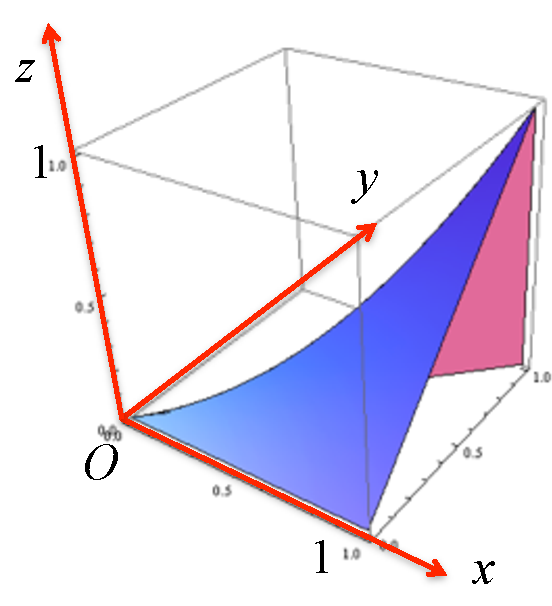
\includegraphics{./images/ch11/xyzC.pdf}}
\end{center}

\fi